\chapter{流形几何与拓扑的恢复}
\label{chap:manifold-recovery}

激光扫描一件雕塑，得到的是成千上万个三维点；记录一个机械臂在各种姿态下的关节读数，得到的是高维空间中的一团点。人们往往相信这些点并非散乱分布，而是落在某个低维的光滑曲面或流形附近。于是问题变成：只凭有限个点，能否知道曲面在每一点朝哪个方向、局部长什么样子，沿曲面从一点走到另一点有多远，以及它有几个分支、几个洞？这些量在前面各章中都是对已知流形定义的，现在流形本身未知，手中只有它的样本。

本章先在第~\ref{sec:mrec-sampling}节建立共同的采样模型：样本多密、观测偏离流形多远、流形自身在环境中弯曲和靠近的程度由可达半径描述，以及这些尺度怎样共同约束邻域的选取。随后分四条线索展开。第~\ref{sec:mrec-tangent}节用邻域内样本的主方向估计切空间，第~\ref{sec:mrec-local-fit}节在估计的平面上拟合图函数，得到连续的局部曲面片。第~\ref{sec:mrec-intrinsic-distance}节用连接邻近样本的图上最短路逼近沿流形的内在距离。

第~\ref{sec:mrec-homology-recovery}节转向拓扑：以样本为球心的球并把离散点变成连续空间，Čech复形用有限组合数据记录它，神经引理和形变收缩把底层流形的同调与有限的线性代数计算联系起来。第~\ref{sec:mrec-persistence}节处理尺度事先未知的情形，让复形随尺度增长，用条形码记录同调信息跨尺度的变化，并证明这种表示对距离扰动稳定。

几条线索各有自己的条件和输出，不能相互替代：局部拟合好不说明拼起来就是流形，同调恢复不需要局部拟合，持久同调的稳定性也不等于它恢复了流形的同调。本章的结论都针对确定的样本与确定的扰动界；样本随机抽取时，满足这些条件的概率有多大，属于统计的问题，留给卷八。所用的流形、切空间与嵌入取自第~\ref{chap:manifold-basics}章和第~\ref{chap:manifold-relations}章，内在距离与曲率取自第~\ref{chap:riemannian-geometry}章，同伦与同调取自第~\ref{chap:homology}章。

\section{采样模型}
\label{sec:mrec-sampling}

要讨论“由样本恢复流形”，先要说清样本与流形是什么关系，以及用什么尺度衡量“足够密”“足够近”“足够平”。本章始终固定一个紧致、无边界的光滑嵌入子流形$M\subseteq\mathbb R^D$，维数为$m$，它可以有有限个连通分支。先讨论样本恰好落在$M$上的情形，再单独加入离开流形的扰动。

有三种容易混淆的距离。环境距离$\lVert\bm x-\bm y\rVert_2$是$\mathbb R^D$中的直线距离，任意两点都能算。内在距离$d_M(\bm p,\bm q)$是第~\ref{chap:riemannian-geometry}章在嵌入诱导度量下定义的距离，只对$M$上的点有意义；两点在不同分支时约定为$+\infty$。样本间距则是样本彼此相隔多远，是样本自身的属性。

打个比方，环境距离是打穿地球的直线隧道，内在距离是沿地表走的路程。两点靠得很近时二者几乎相同，隔得远时可以相差很多。本章的很多论证，都是在“小尺度上二者接近”这一点上做文章。

本节引入的覆盖精度和可达半径是对$M$与样本关系的假设，用来陈述“在什么条件下恢复成立”。它们不能从有限样本中准确读出：只看样本，无法知道流形在两个样本之间是否藏着一个小褶皱。

\subsection{样本覆盖}
\label{sec:mrec-coverage}

样本能否代表流形，首先要看流形上有没有远离所有样本的地方。设$P=\{\bm p_1,\ldots,\bm p_n\}\subseteq M$是有限样本。

\begin{definition}[稠密样本]
\label{def:mrec-dense-sample}
设$\delta>0$。若对每个$\bm x\in M$都存在$\bm p\in P$使$\lVert\bm x-\bm p\rVert_2<\delta$，则称$P$是$M$的$\delta$\term{稠密样本}（dense sample）。
\end{definition}

把每个样本换成半径$\delta$的开球，定义说的就是这些球盖住了整个$M$。函数$\bm x\mapsto\min_{\bm p\in P}\lVert\bm x-\bm p\rVert_2$在紧集$M$上连续，所以有最大值，记为
\begin{equation}
 \delta_P=\max_{\bm x\in M}\ \min_{\bm p\in P}\lVert\bm x-\bm p\rVert_2 ,
 \label{eq:mrec-covering-radius}
\end{equation}
称为$P$的覆盖精度。它是流形上最孤立的那一点到最近样本的距离，$P$是$\delta$稠密样本当且仅当$\delta_P<\delta$。图~\ref{fig:mrec-coverage}(a)画的是一条闭曲线和覆盖它的小圆盘。

单位圆上取$n$个等距样本，可以直接算出覆盖精度。最孤立的点是相邻两样本之间的弧中点，它到最近样本的圆心角是$\pi/n$，对应的弦长就是
\[
 \delta_P=2\sin\frac{\pi}{2n}.
\]
于是$n=6$时$\delta_P=2\sin15^\circ\approx0.518$，$n=24$时$\delta_P=2\sin3.75^\circ\approx0.131$。这两组数后面会反复用到。

定义用的是环境距离。同一对点的环境距离不超过内在距离，所以内在意义下稠密蕴含环境意义下稠密；反过来不一定，因为环境中靠近的两点沿流形可能很远。

\begin{BookInlineFigure}
  \centering
  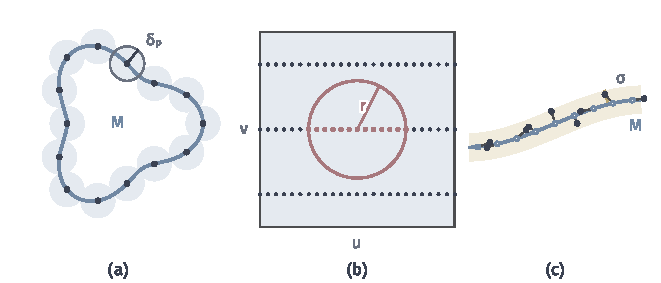
\includegraphics[width=112mm]{figures/04-spaces-measures-and-geometry/04-manifolds/matplotlib/mrec-coverage/figure.pdf}
  \caption{样本与流形的三种关系。(a) 曲线上$14$个样本（黑点），半径取覆盖精度$\delta_P$的圆盘把曲线盖满。(b) 一块平坦区域上的三条水平样本线，全域稠密，但红圈内的样本全在一条线上，只提供$u$方向的信息。(c) 观测（黑点）由真实采样点（空心点）沿任意方向偏移不超过$\sigma$，都落在曲线的$\sigma$管状邻域（浅黄）内。}
  \label{fig:mrec-coverage}
\end{BookInlineFigure}

\paragraph{局部邻域}

后面的局部计算都在某个位置附近进行。对选定的中心$\bm c\in\mathbb R^D$和半径$r>0$，记邻域样本为
\begin{equation}
 N_r(\bm c)=\{\bm p\in P:\lVert\bm p-\bm c\rVert_2\leq r\}.
 \label{eq:mrec-neighborhood}
\end{equation}
中心可以是一个样本，也可以是需要估计的任意位置。选邻域有定半径和定点数两种做法。本章采用定半径，因为$r$是一个明确的几何尺度，可以直接与覆盖精度和后面的可达半径比较；按点数选取时，各处的半径随采样疏密而变。

\paragraph{全域稠密与方向分布}

全域稠密只说明每一点附近都有样本，并不说明在某个邻域内，样本沿流形的各个方向都铺开了。设$M$的一块区域是平的，用坐标$(u,v)\in[0,1]^2$表示，例如平环面上的一小块。在这块区域上只沿三条水平线$v=\tfrac16,\tfrac12,\tfrac56$取样，每条线上的样本间距为$\tfrac1{24}$，如图~\ref{fig:mrec-coverage}(b)。

这组样本在全域上相当密。最孤立的点在两条水平线的正中间，又在两个相邻样本的正中间，所以
\[
 \delta_P=\sqrt{\bigl(\tfrac16\bigr)^2+\bigl(\tfrac1{48}\bigr)^2}\approx0.168 .
\]

现在以水平线上的一个样本为中心取半径$r=0.25$。相邻水平线的间隔是$\tfrac13>r$，所以邻域里的$13$个样本全在同一条水平线上。它们沿$u$方向铺开，完全不提供$v$方向的信息，后面的局部线性拟合会得到秩不足的矩阵。

所以全域稠密不能单独保证局部拟合的秩和条件数，邻域内的方向分布要另作要求。第~\ref{sec:mrec-tangent-error}节把这一要求写成局部矩阵的特征值条件。

\subsection{观测扰动}
\label{sec:mrec-noise}

实际观测很少恰好落在流形上。把第$i$个观测写成
\begin{equation}
 \bm x_i=\bm p_i+\bm e_i,\qquad\bm p_i\in M,\quad\lVert\bm e_i\rVert_2\leq\sigma ,
 \label{eq:mrec-noise-model}
\end{equation}
其中$\bm p_i$是看不到的真实采样位置，$\bm e_i$是环境空间中的有界扰动，方向任意，如图~\ref{fig:mrec-coverage}(c)。

这一模型把两种误差分开记录：真实采样点的覆盖精度$\delta_P$描述流形上有没有空缺，扰动界$\sigma$描述观测离开流形多远。由三角不等式，每个观测到$M$的距离不超过$\sigma$；而$M$上任一点先走到最近的真实采样点，再走到对应的观测，所以
\[
 \min_i\lVert\bm x-\bm x_i\rVert_2\leq\delta_P+\sigma,\qquad\bm x\in M.
\]

扰动改变了能够谈论的对象。$\bm x_i\notin M$时，$\bm x_i$处的切空间没有定义，$d_M(\bm x_i,\bm x_j)$也没有定义，能估计的只是附近真实位置处的量。所以无噪声的结论不能直接搬过来，每个结论都要重新说明$\sigma$进入哪里。

不同的任务对$\sigma$的要求也不同。邻域选择只受环境距离影响，每个成对距离至多变化$2\sigma$。局部拟合要求$\sigma$相对邻域半径小，才能把法向噪声与沿流形的展开区分开。拓扑恢复要求$\sigma$相对流形本身的尺度小，否则噪声可能填掉细小的孔洞。后面各节分别处理。

本章把扰动看成确定的有界量，只问“给定这些界，结论是否成立”。若样本按某个分布随机抽取、噪声是随机变量，则覆盖精度与扰动界都变成随机量，要估计它们以多大概率不超过给定值，可参考\BookChapterRef{chap:finite-sample-error-bounds}{卷八第4章“有限样本的误差上界”}。

\subsection{可达半径}
\label{sec:mrec-reach}

覆盖精度只说明样本多密，还缺一个描述流形自身形状的尺度：样本要密到什么程度，才算“相对于流形足够密”？直观上，流形弯得越厉害，或者它的不同部分靠得越近，所需的样本就越密。这两种情况可以用同一个量刻画。

对$\bm x\in\mathbb R^D$，记$\bm x$到$M$的距离为
\[
 \operatorname{dist}(\bm x,M)=\min_{\bm p\in M}\lVert\bm x-\bm p\rVert_2 .
\]
由$M$紧致，最小值可以取到，取到最小值的点称为$\bm x$在$M$上的最近点。$M$上的点的最近点是它自己；离开$M$以后，最近点可能不唯一，例如平面上单位圆的圆心到圆上每一点的距离都是$1$。

把$M$向外加粗，记
\[
 M^r=\{\bm x\in\mathbb R^D:\operatorname{dist}(\bm x,M)<r\}.
\]
可以想象从$M$出发同时向四面八方“长肉”，$M^r$是长到厚度$r$时的形状。厚度很小时，$M^r$里的每一点都能找回唯一的出发点；厚度增大，从不同地方长出来的部分迟早相撞，相撞处的点就有了两个最近点。可达半径就是这个相撞发生之前的最大厚度。

\begin{definition}[可达半径]
\label{def:mrec-reach}
$M$的\term{可达半径}（reach）定义为
\begin{equation}
 \tau=\sup\{r\geq0:M^r\text{中每一点在}M\text{上都有唯一最近点}\}.
 \label{eq:mrec-reach}
\end{equation}
\end{definition}

半径为$R$的圆的可达半径为$R$：圆心以外的每一点都有唯一最近点，即沿径向的那一点，而圆心离圆的距离恰为$R$。对紧致无边界的光滑嵌入子流形总有$\tau>0$，这是管状邻域定理的推论，证明可查阅Federer关于曲率测度的论文。

在$M^\tau$内，可以定义最近点投影$\pi$：$\pi(\bm x)$是$\bm x$在$M$上唯一的最近点。这个投影是连续的。设$\bm x_k\to\bm x$都在$M^\tau$中，由$M$紧致，$\pi(\bm x_k)$的任一收敛子列有极限$\bm z\in M$，并且
\[
 \lVert\bm x-\bm z\rVert_2=\lim_k\lVert\bm x_k-\pi(\bm x_k)\rVert_2=\lim_k\operatorname{dist}(\bm x_k,M)=\operatorname{dist}(\bm x,M).
\]
所以$\bm z$是$\bm x$的最近点，由唯一性$\bm z=\pi(\bm x)$。每个收敛子列的极限都是$\pi(\bm x)$，于是$\pi(\bm x_k)\to\pi(\bm x)$。

最近点还有一条一阶条件：$\bm x-\pi(\bm x)$与$M$在$\pi(\bm x)$处的切空间垂直。这是因为沿$M$上过$\pi(\bm x)$的任一曲线，到$\bm x$的距离平方在$\pi(\bm x)$处取最小值，导数为零。

\paragraph{限制可达半径的三种情形}

可达半径同时受三种因素限制，图~\ref{fig:mrec-reach-limits}分别画出了它们。

第一种是局部弯曲。图中是长半轴$2$、短半轴$1$的椭圆。在长轴端点$(2,0)$处曲率半径为$b^2/a=\tfrac12$，沿内法向走到曲率中心$(\tfrac32,0)$，这里是所有“最近点不唯一”的位置组成的线段的端点。一般地，曲线上曲率为$\kappa$的点使$\tau\leq1/\kappa$，圆的情形正是$\tau=R=1/\kappa$，椭圆的可达半径正是$\tfrac12$。

第二种是同一分支的不同部分相互接近。图~\ref{fig:mrec-reach-limits}(b)的闭曲线在中部收窄，两股相距$2b$，那里的曲率并不大，但中点$\bm z$到上下两股的距离相等，有两个最近点，所以$\tau\leq b$。第三种是不同分支相互接近，这时分支之间的距离直接控制可达半径。

\begin{BookInlineFigure}
  \centering
  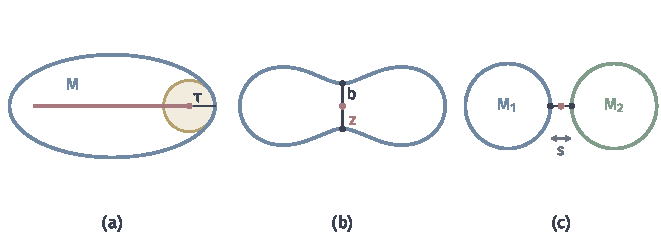
\includegraphics[width=112mm]{figures/04-spaces-measures-and-geometry/04-manifolds/matplotlib/mrec-reach-limits/figure.pdf}
  \caption{限制可达半径的三种情形。(a) 椭圆内部红色线段上的点都有两个或更多最近点，线段端点是长轴端点的曲率中心，到曲线的距离$\tau=\tfrac12$是这一位置的曲率半径。(b) 曲线中部收窄，中点$\bm{z}$有上下两个最近点，$\tau\leq b$。(c) 两个分支相距$s$，中点（红）同样有两个最近点，$\tau\leq s/2$。}
  \label{fig:mrec-reach-limits}
\end{BookInlineFigure}

\begin{lemma}[不同分支的间隔]
\label{lem:mrec-component-gap}
$M$的任意两个不同连通分支之间的环境距离不小于$2\tau$。
\end{lemma}
\begin{proof}
紧致流形只有有限个分支，每个分支紧致。所以在所有“属于不同分支”的点对中，环境距离的最小值$s$可以由某对$\bm p\in M_1$、$\bm q\in M_2$取到。

假设$s<2\tau$，取中点$\bm z=\tfrac12(\bm p+\bm q)$，则$\operatorname{dist}(\bm z,M)\leq s/2<\tau$，$\bm z$有唯一最近点$\bm w$。若$\lVert\bm z-\bm w\rVert_2=s/2$，则$\bm p,\bm q$都是$\bm z$的最近点，与唯一性矛盾，所以
\[
 \lVert\bm z-\bm w\rVert_2<\frac s2 .
\]

由三角不等式，
\[
 \lVert\bm p-\bm w\rVert_2\leq\lVert\bm p-\bm z\rVert_2+\lVert\bm z-\bm w\rVert_2<s,
\]
同样$\lVert\bm q-\bm w\rVert_2<s$。而$\bm w$所在的分支至少与$M_1$、$M_2$之一不同，这就找到了一对距离小于$s$的不同分支的点，与$s$的最小性矛盾。所以$s\geq2\tau$。
\end{proof}

\paragraph{可达半径控制的局部几何}

后面要用可达半径控制两件事：流形离切平面有多远，沿流形的路程比直线长多少。先看一个几何事实。在$\bm q\in M$处取单位法向量$\bm v$，沿它走一小段距离$s$，到达的点$\bm q+s\bm v$的最近点应当还是$\bm q$。下面的引理说，这一点一直保持到$s=\tau$。

\begin{lemma}[法向线段]
\label{lem:mrec-normal-segment}
设$\bm q\in M$，$\bm v$是$M$在$\bm q$处的单位法向量，$0\leq s<\tau$，则$\pi(\bm q+s\bm v)=\bm q$。
\end{lemma}
\begin{proof}
记$M$的法丛为
\[
 N=\{(\bm a,\bm w):\bm a\in M,\ \bm w\perp T_{\bm a}M\}.
\]
用局部的法向标准正交标架作坐标，可知$N$是$D$维流形。定义映射
\[
 \Phi:M^\tau\to N,\qquad\Phi(\bm x)=\bigl(\pi(\bm x),\ \bm x-\pi(\bm x)\bigr).
\]
由最近点的一阶条件，$\Phi$确实落在$N$中；由$\pi$连续，$\Phi$连续。

$\Phi$是单射，因为由$\Phi(\bm x)$相加两个分量就得到$\bm x$。$M^\tau$是$\mathbb R^D$的开集，$N$是$D$维流形，由Brouwer的区域不变性定理，连续单射$\Phi$的像$\Phi(M^\tau)$是$N$的开集。

令$A=\{s\in[0,\tau):\pi(\bm q+s\bm v)=\bm q\}$。首先$0\in A$。由$\pi$连续，$A$在$[0,\tau)$中是闭的。

再看$A$是开的。设$s\in A$，则
\[
 (\bm q,s\bm v)=\Phi(\bm q+s\bm v)\in\Phi(M^\tau).
\]
$\Phi(M^\tau)$是开集，所以当$s'$靠近$s$时$(\bm q,s'\bm v)$也在其中，即存在$\bm y\in M^\tau$使
\[
 \Phi(\bm y)=(\bm q,s'\bm v).
\]
相加两个分量得$\bm y=\bm q+s'\bm v$，并且$\pi(\bm y)=\bm q$，这就是$s'\in A$。

$[0,\tau)$连通，$A$既开又闭且非空，所以$A=[0,\tau)$。
\end{proof}

这条引理有一幅很直观的图像：在$\bm q$处沿法向放一个半径略小于$\tau$的球，球心是$\bm q+s\bm v$，引理说球内部不含$M$的点。可以想象一个半径为$\tau$的球沿$M$滚动，它能贴着$M$走遍每一点而不被挤开，如图~\ref{fig:mrec-rolling-ball}(a)。把这幅图写成不等式，就得到流形偏离切平面的界。

\begin{lemma}[法向偏离]
\label{lem:mrec-normal-distance}
对任意$\bm p,\bm q\in M$，$\bm q-\bm p$到切空间$T_{\bm p}M$的距离满足
\begin{equation}
 \operatorname{dist}(\bm q-\bm p,\ T_{\bm p}M)\leq\frac{\lVert\bm q-\bm p\rVert_2^2}{2\tau}.
 \label{eq:mrec-reach-normal}
\end{equation}
\end{lemma}
\begin{proof}
把$\bm q-\bm p$分解为切向部分与法向部分$\bm n$，式~\eqref{eq:mrec-reach-normal}的左端就是$\lVert\bm n\rVert_2$。$\bm n=\bm 0$时不用证，否则令$\bm v=\bm n/\lVert\bm n\rVert_2$。

对$0<s<\tau$，由引理~\ref{lem:mrec-normal-segment}，$\bm p$是$\bm p+s\bm v$的最近点，所以$\bm q$到它的距离不小于$s$：
\[
 \lVert\bm q-\bm p-s\bm v\rVert_2^2\geq s^2 .
\]
展开左端，并注意切向部分与$\bm v$垂直，$\bm q-\bm p$在$\bm v$上的分量就是$\lVert\bm n\rVert_2$，得
\[
 \lVert\bm q-\bm p\rVert_2^2-2s\lVert\bm n\rVert_2\geq0 .
\]
令$s\to\tau$，就得到式~\eqref{eq:mrec-reach-normal}。
\end{proof}

\begin{BookInlineFigure}
  \centering
  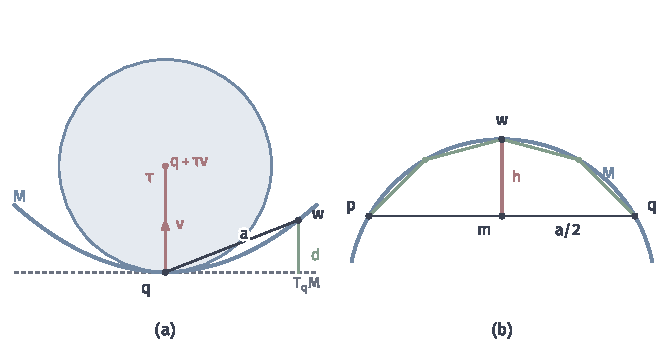
\includegraphics[width=112mm]{figures/04-spaces-measures-and-geometry/04-manifolds/matplotlib/mrec-rolling-ball/figure.pdf}
  \caption{可达半径的两个局部结论。(a) 半径为$\tau$的球（浅蓝）贴在$M$上，内部不含$M$的点，由此$\bm w$到切线的距离$d\leq a^2/(2\tau)$，其中$a$是$\bm q$到$\bm w$的弦长。(b) 半径为$\tau$的圆是引理~\ref{lem:mrec-midpoint}的极端情形：弦$\bm p\bm q$的中点$\bm m$投影到$\bm w$，两段新弦（绿）的长度恰为$2\tau\sin(\theta/2)$；继续细分，折线长度趋于弧长$2\tau\theta$。}
  \label{fig:mrec-rolling-ball}
\end{BookInlineFigure}

要控制沿流形的路程，办法是不断取弦的中点并投影回$M$，每投影一次，弦就更贴近流形，如图~\ref{fig:mrec-rolling-ball}(b)。下面的引理把一次投影的效果算清楚：它对中点的最近点用两次式~\eqref{eq:mrec-reach-normal}，把$\bm p$、$\bm q$到它的距离一起控制住。

\begin{lemma}[中点投影]
\label{lem:mrec-midpoint}
设$\bm p,\bm q\in M$，$a=\lVert\bm p-\bm q\rVert_2<2\tau$，把$a$写成$2\tau\sin\theta$，$\theta\in[0,\pi/2)$。则存在$\bm w\in M$，使
\begin{equation}
 \max\bigl(\lVert\bm p-\bm w\rVert_2,\ \lVert\bm q-\bm w\rVert_2\bigr)\leq2\tau\sin\frac\theta2 .
 \label{eq:mrec-midpoint}
\end{equation}
\end{lemma}
\begin{proof}
令$\bm m=\tfrac12(\bm p+\bm q)$，它到$\bm p$的距离是$a/2$，所以$\operatorname{dist}(\bm m,M)\leq a/2<\tau$，可取最近点$\bm w=\pi(\bm m)$，记$h=\lVert\bm m-\bm w\rVert_2$。

$h=0$时$\bm w=\bm m$，到两端的距离都是$a/2$，而
\[
 \frac a2=\tau\sin\theta\leq2\tau\sin\frac\theta2 ,
\]
结论成立。下设$h>0$。

令$\bm v=(\bm m-\bm w)/h$，由一阶条件，$\bm v$是$\bm w$处的单位法向量。记$c=\langle\bm p-\bm m,\bm v\rangle$，由对称性不妨设$c\geq0$，再记$A=a^2/4+h^2$。

按$\bm p-\bm w=(\bm p-\bm m)+(\bm m-\bm w)$展开，并用$\bm q-\bm m=-(\bm p-\bm m)$，得
\[
 \lVert\bm p-\bm w\rVert_2^2=A+2hc,\qquad\lVert\bm q-\bm w\rVert_2^2=A-2hc .
\]
同时，$\bm p-\bm w$在$\bm v$上的分量是$h+c$，$\bm q-\bm w$在$\bm v$上的分量是$h-c$。

对$\bm p$、$\bm w$与$\bm q$、$\bm w$分别用式~\eqref{eq:mrec-reach-normal}，得
\[
 h+c\leq\frac{A+2hc}{2\tau},\qquad h-c\leq\frac{A-2hc}{2\tau}.
\]
两式相加，得到
\[
 2\tau h\leq A,\qquad\text{即}\quad h^2-2\tau h+\frac{a^2}4\geq0 .
\]
又$h\leq a/2<\tau$，所以$h$不超过这个二次式的较小根：
\[
 h\leq h_*=\tau-\sqrt{\tau^2-a^2/4}=\tau(1-\cos\theta).
\]

从第一式解出$c$，由$\tau-h>0$，
\[
 c\leq\frac{A-2\tau h}{2(\tau-h)}.
\]
代回$\lVert\bm p-\bm w\rVert_2^2=A+2hc$，整理得
\[
 \lVert\bm p-\bm w\rVert_2^2\leq g(h)=\frac{\tau(a^2/4-h^2)}{\tau-h}.
\]

对$g$求导，
\[
 g'(h)=\frac{\tau(h^2-2\tau h+a^2/4)}{(\tau-h)^2}\geq0,\qquad 0\leq h\leq h_*,
\]
所以$g(h)\leq g(h_*)$。用$a/2=\tau\sin\theta$代入，
\[
 g(h_*)=\frac{\tau\cdot2\tau^2\cos\theta(1-\cos\theta)}{\tau\cos\theta}=2\tau^2(1-\cos\theta)=\bigl(2\tau\sin\tfrac\theta2\bigr)^2 .
\]
由$c\geq0$，$\bm q$到$\bm w$的距离不超过$\bm p$到$\bm w$的距离，所以两段距离都不超过$2\tau\sin(\theta/2)$。
\end{proof}

把式~\eqref{eq:mrec-reach-normal}和反复投影的结果写在一起，就是后面各节反复使用的两条局部推论。

\begin{theorem}[可达半径的局部推论]
\label{thm:mrec-reach-consequences}
设$M$的可达半径为$\tau>0$，$\bm p,\bm q\in M$。则$\bm q-\bm p$到$T_{\bm p}M$的距离满足式~\eqref{eq:mrec-reach-normal}。若$\lVert\bm p-\bm q\rVert_2<2\tau$，则$\bm p,\bm q$属于同一分支，并且
\begin{equation}
 d_M(\bm p,\bm q)\leq2\tau\arcsin\frac{\lVert\bm p-\bm q\rVert_2}{2\tau}.
 \label{eq:mrec-reach-arc}
\end{equation}
\end{theorem}

\begin{proof}
第一条就是引理~\ref{lem:mrec-normal-distance}。再看第二条，由引理~\ref{lem:mrec-component-gap}，$\bm p,\bm q$在同一分支。把$\lVert\bm p-\bm q\rVert_2$写成$2\tau\sin\theta$，$\theta<\pi/2$。对$\bm p,\bm q$用引理~\ref{lem:mrec-midpoint}得到$\bm w$，再对$(\bm p,\bm w)$和$(\bm w,\bm q)$分别用一次，如此重复$k$轮。

每轮把相邻两点弦长对应的角减半，$k$轮后得到$M$上$2^k+1$个点，相邻点的距离都不超过$2\tau\sin(\theta/2^k)$，这些弦长的总和不超过
\[
 2^k\cdot2\tau\sin\frac\theta{2^k}\leq2\tau\theta .
\]
在紧致流形上，$\lVert\bm x-\bm y\rVert_2\to0$时$d_M(\bm x,\bm y)/\lVert\bm x-\bm y\rVert_2$一致趋于$1$，因为$M$在小尺度上是斜率很小的图。所以对任意$\eta>0$，$k$足够大时
\[
 d_M(\bm p,\bm q)\leq(1+\eta)\,2\tau\theta .
\]
令$\eta\to0$，并由$\theta=\arcsin(\lVert\bm p-\bm q\rVert_2/2\tau)$，得式~\eqref{eq:mrec-reach-arc}。
\end{proof}

两条结论在圆上都取等号。在半径为$R$的圆上，取$\bm p$处的切线为水平方向，$\bm q$对应圆心角$\theta$，则法向分量为$R(1-\cos\theta)$，弦长的平方为$2R^2(1-\cos\theta)$，式~\eqref{eq:mrec-reach-normal}取等号；弦长$s$对应的弧长为$2R\arcsin(s/2R)$，式~\eqref{eq:mrec-reach-arc}也取等号。所以这两个估计不能再改进。

第一条说，在半径为$r$的邻域内，流形偏离切平面至多$r^2/(2\tau)$，相对于邻域半径的比值是$r/(2\tau)$。第二条说，环境距离小于$2\tau$的两点，沿流形的距离不会比直线长太多：$\lVert\bm p-\bm q\rVert_2\leq\tau$时，比值至多为$2\arcsin\tfrac12=\pi/3\approx1.047$。

第一条还给出弯曲的上界。设$\gamma$是$M$上过$\bm p$的单位速度测地线，$\gamma(s)-\bm p$的切向部分近似$s\gamma'(0)$，法向部分近似$\tfrac12s^2\gamma''(0)$，而弦长近似$s$。代入式~\eqref{eq:mrec-reach-normal}，令$s\to0$，得$\lVert\gamma''(0)\rVert_2\leq1/\tau$，即每条测地线作为$\mathbb R^D$中的曲线，曲率都不超过$1/\tau$。

\subsection{邻域尺度}
\label{sec:mrec-neighborhood-scale}

局部计算的成败，关键在邻域半径$r$的选取。图~\ref{fig:mrec-scale}用同一组带噪声的样本比较了三种半径。

$r$过小时，邻域内的样本太少，甚至只有中心自己。即使样本不少，若$r$与扰动界$\sigma$同量级，邻域内样本的散布主要来自噪声，看不出流形的方向，如图(a)。所以$r$要明显大于覆盖精度$\delta_P$和$\sigma$。

$r$过大时出现另外两类问题。由定理~\ref{thm:mrec-reach-consequences}，流形在邻域内偏离切平面可达$r^2/(2\tau)$，$r$与$\tau$可比时这一偏离与邻域本身一样大，局部已不能看成平的。另外，$r$超过两股的间隔时，邻域会同时包含两股的样本，如图(c)，它们在环境中靠近，沿流形却相距很远。

由定理~\ref{thm:mrec-reach-consequences}的第二条，$r<2\tau$时邻域内的点都属于同一分支；要使局部线性近似可靠，还要$r$远小于$\tau$。所以分析的范围大致是
\begin{equation}
 \delta_P,\ \sigma\ll r\ll\tau .
 \label{eq:mrec-scale-range}
\end{equation}

\begin{BookInlineFigure}
  \centering
  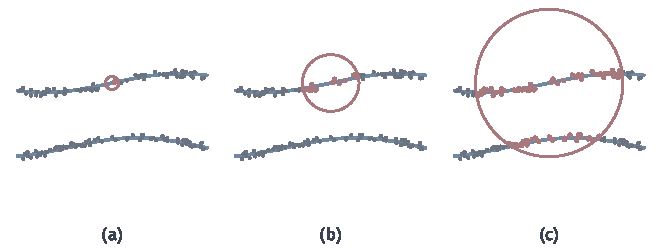
\includegraphics[width=112mm]{figures/04-spaces-measures-and-geometry/04-manifolds/matplotlib/mrec-scale/figure.pdf}
  \caption{同一组带噪声的样本在三种邻域半径下的情形，两条蓝线是流形的两股，红点是邻域内的样本。(a) 半径与噪声同量级，邻域内只有零星几个点。(b) 半径适中，邻域内的样本沿一股展开。(c) 半径超过两股的间隔，邻域混入另一股的样本。}
  \label{fig:mrec-scale}
\end{BookInlineFigure}

\paragraph{嵌入弯曲决定局部线性误差}

第~\ref{chap:riemannian-geometry}章区分了内在曲率与嵌入弯曲。半径为$\rho$的圆柱面内在地是平的，可以展开成平面而不改变任何长度，如图~\ref{fig:mrec-cylinder}(b)；但它在$\mathbb R^3$中弯曲，可达半径为$\rho$，切平面只在一条母线上贴着它，如图~\ref{fig:mrec-cylinder}(a)。

取$\rho=1$，沿圆周方向取一点，弦长$r=0.5$，它对应的圆心角$\theta$满足$2\sin(\theta/2)=0.5$，到切平面的距离是
\[
 1-\cos\theta=\frac{r^2}{2\rho}=0.125 .
\]
内在曲率为零并没有让这一偏离消失；沿母线方向偏离却恰好是零。这说明局部线性误差首先由环境中的嵌入形状决定，可达半径度量的正是这一形状，内在曲率是另一回事。

\begin{BookInlineFigure}
  \centering
  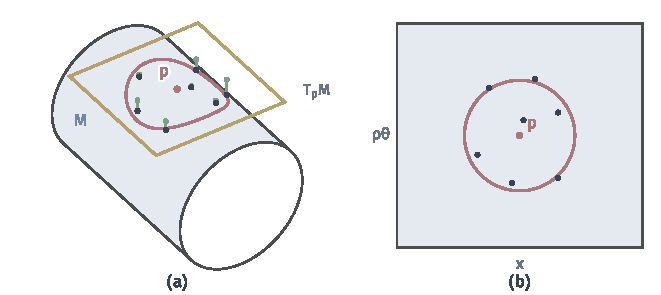
\includegraphics[width=112mm]{figures/04-spaces-measures-and-geometry/04-manifolds/matplotlib/mrec-cylinder/figure.pdf}
  \caption{圆柱面的内在几何与嵌入形状。(a) 点$\bm{p}$处的切平面（黄色框）与红圈内的邻域，绿色线段是样本（黑点）到切平面的法向偏离，沿圆周方向偏离最大。(b) 把圆柱面沿母线剪开摊平，同一邻域和样本成为平面上的圆盘和点，长度不变，内在曲率为零。}
  \label{fig:mrec-cylinder}
\end{BookInlineFigure}

反过来，即使嵌入弯曲很小，邻域内样本的方向覆盖仍需单独核验，第~\ref{sec:mrec-coverage}节的水平线采样就是例子。选定$r$以后，邻域应同时满足三条：足够小，使弯曲可以忽略；足够大，使样本数和散布压过噪声；样本在各个切向上都有展开。

\section{切空间估计}
\label{sec:mrec-tangent}

切空间是流形在一点处的线性近似。第~\ref{chap:manifold-basics}章用曲线的速度或局部坐标定义它，第~\ref{chap:manifold-relations}章说明嵌入子流形的切空间是环境空间的线性子空间。现在只有样本，没有局部坐标，也没有曲线。

本节先说明切空间在什么意义上近似流形，再把这一近似落实为有限样本上的子空间拟合，最后分析拟合误差。局部主成分分析是一种估计方法，它的输出只有在几何近似成立时才是切空间的近似，不能反过来把它当作切空间的定义。

\subsection{切向近似}
\label{sec:mrec-tangent-approx}

在点$\bm p\in M$附近，把环境空间分解为切空间$T=T_{\bm p}M$与它的正交补，即法空间$T^\perp$。把$M$上的点正交投影到$T$，这个映射在$\bm p$处的导数是$T$上的恒等映射，由反函数定理在局部可逆。

它的逆就给出参数化$\bm u\mapsto\bm p+\bm u+g(\bm u)$。也就是说，存在$\bm0$在$T$中的邻域$W$和$C^2$映射$g:W\to T^\perp$，使$M$在$\bm p$附近的部分恰为
\begin{equation}
 \{\bm p+\bm u+g(\bm u):\bm u\in W\},\qquad g(\bm0)=\bm0,\quad Dg(\bm0)=\bm0 .
 \label{eq:mrec-local-graph}
\end{equation}
这里的$g$就是图~\ref{fig:mrec-cylinder}(a)中那些绿色线段的长度和方向：从切平面上的$\bm u$沿法向走$g(\bm u)$，就回到流形。

条件$Dg(\bm0)=\bm0$表达的正是切空间的局部线性作用：沿切向移动$\bm u$，流形在法向上的偏离没有一阶项。对$C^2$的$g$，若它的二阶导数在$W$中某个凸邻域上的范数不超过$K$，由多元Taylor公式，在这个邻域中
\[
 \lVert g(\bm u)\rVert_2\leq\frac K2\lVert\bm u\rVert_2^2 .
\]
多元Taylor展开与余项可参考\BookChapterRef{chap:multivariate-differentiation}{卷二第17章“多元函数微分”}。这个界依赖图函数的坐标，式~\eqref{eq:mrec-reach-normal}给出不依赖坐标的同类界，只用到可达半径。

这是邻域尺度下的近似，不是全局平面表示。以半径为$R$的圆为例，在最低点处取水平切线，图函数是
\[
 g(u)=R-\sqrt{R^2-u^2}=\frac{u^2}{2R}+O(u^4),
\]
二次项正是曲率决定的偏离。但这个表示只在$\lvert u\rvert<R$时有定义，越过左右两端，圆就不再是水平线上的图，切线近似也随之失去意义。

\subsection{局部PCA}
\label{sec:mrec-local-pca}

切向近似说明，在小邻域内，流形上的点主要沿切向展开，法向偏离是二阶小量。于是可以把邻域内的样本当作一团数据，寻找它们展开最多的$m$个方向。这里假定流形的维数$m$已经指定，邻域也已选定，记其中的观测为$\bm x_1,\ldots,\bm x_k$。

\paragraph{局部协方差与主方向}

计算局部质心与局部协方差矩阵
\begin{equation}
 \overline{\bm x}=\frac1k\sum_{j=1}^k\bm x_j,\qquad
 \bm C=\frac1k\sum_{j=1}^k(\bm x_j-\overline{\bm x})(\bm x_j-\overline{\bm x})^\top .
 \label{eq:mrec-local-covariance}
\end{equation}
$\bm C$是$D$阶对称半正定矩阵。取它最大的$m$个特征值对应的标准正交特征向量，排成$\widehat{\bm U}\in\mathbb R^{D\times m}$，其列空间$\widehat S$就是切空间的估计。这一方法称为\term{局部主成分分析}（local principal component analysis）。

主方向的意义来自一个最优性：$\widehat S$在全部$m$维线性子空间中，使中心化样本到子空间的平方距离和最小。记$\bm y_j=\bm x_j-\overline{\bm x}$，取$S$的一组标准正交基排成$\bm V\in\mathbb R^{D\times m}$。$\bm y_j$到$S$的距离的平方，是它的长度平方减去投影长度的平方，所以
\[
 \begin{aligned}
 \sum_j\operatorname{dist}(\bm y_j,S)^2
 &=\sum_j\lVert\bm y_j\rVert_2^2-\sum_j\lVert\bm V^\top\bm y_j\rVert_2^2\\
 &=k\operatorname{tr}\bm C-k\operatorname{tr}(\bm V^\top\bm C\bm V).
 \end{aligned}
\]
第一项与$S$无关，所以最小化距离和等价于最大化$\operatorname{tr}(\bm V^\top\bm C\bm V)$。它的最大值是前$m$个特征值之和，由前$m$个特征向量取到，这一迹极值可参考\BookChapterRef{chap:matrix-approximation}{卷二第15章“矩阵逼近”}。在全部$m$维仿射平面中，到样本的平方距离和最小的是$\overline{\bm x}+\widehat S$。

\paragraph{子空间、基与平面}

这里有三个不同的对象。$\widehat S$是方向子空间，是对$T_{\bm p}M$的估计。$\widehat{\bm U}$只是它的一组标准正交基，右乘任何$m$阶正交矩阵仍是同一个子空间的基，所以比较估计与真值时只能比较子空间，例如用主夹角。$\overline{\bm x}+\widehat S$是拟合平面，它还带有位置信息，而局部质心一般不在流形上，也不等于$\bm p$。

\paragraph{矩阵的秩不是流形的维数}

有限样本的协方差矩阵的秩不能直接当作真实维数。带噪声时$\bm C$一般满秩，秩等于$\min(D,k-1)$，与$m$无关；无噪声时，流形的弯曲也使样本不落在任何$m$维平面上，$\bm C$的秩仍可能大于$m$。

例~\ref{ex:mrec-one-sided}的三个点在一条曲线上，$m=1$，却算出秩为$2$的$\bm C$，两个特征值约为$4.43\times10^{-2}$和$2.0\times10^{-4}$。谱中前$m$个特征值明显大于其余，可以作为维数的线索，但要把它当作判断，就必须结合下一小节的误差分析说明“明显”的界限。本节始终把$m$看作已知。

\subsection{切空间估计的误差}
\label{sec:mrec-tangent-error}

现在估计$\widehat S$偏离$T=T_{\bm p}M$多远。误差有三个来源：流形在邻域内的弯曲，邻域内样本在切向上的分布，以及观测扰动。下面把它们分别写进局部协方差矩阵，再用特征子空间的扰动界控制方向的偏离。

所用的工具是\BookChapterRef{chap:condition-and-spectral-perturbation}{卷二第7章“条件数与谱扰动”}中的Davis--Kahan谱隙界。设对称矩阵$\bm C_0$扰动为$\bm C=\bm C_0+\bm E$，$\gamma=\lambda_m(\bm C_0)-\lambda_{m+1}(\bm C)>0$，则两者的前$m$个特征子空间的最大主夹角$\theta_{\max}$满足
\begin{equation}
 \sin\theta_{\max}\leq\frac{\lVert\bm E\rVert_2}{\gamma}.
 \label{eq:mrec-davis-kahan}
\end{equation}

\paragraph{误差的分解}

设邻域中观测$\bm x_j$对应的真实采样点$\bm p_j$满足$\lVert\bm p_j-\bm p\rVert_2\leq r$。把$\bm p_j-\bm p$分解为切向部分$\bm u_j\in T$与法向部分$\bm n_j\in T^\perp$，在图表示成立的范围内$\bm n_j=g(\bm u_j)$，于是
\[
 \bm x_j=\bm p+\bm u_j+\bm n_j+\bm e_j,\qquad\lVert\bm e_j\rVert_2\leq\sigma .
\]

用上划线表示邻域平均，记
\[
 \bm a_j=\bm u_j-\overline{\bm u}\in T,\qquad
 \bm b_j=(\bm n_j-\overline{\bm n})+(\bm e_j-\overline{\bm e}).
\]
则$\bm x_j-\overline{\bm x}=\bm a_j+\bm b_j$，切向展开全部在$\bm a_j$里，弯曲和噪声全部在$\bm b_j$里。代入式~\eqref{eq:mrec-local-covariance}，
\[
 \bm C=\bm C_0+\bm E,\qquad\bm C_0=\frac1k\sum_j\bm a_j\bm a_j^\top ,
\]
\[
 \bm E=\frac1k\sum_j\bigl(\bm a_j\bm b_j^\top+\bm b_j\bm a_j^\top+\bm b_j\bm b_j^\top\bigr).
\]

$\bm C_0$的像在$T$中，在$T^\perp$上为零。记它在$T$上的最小特征值为$\lambda_T$，它度量样本在最不充分的那个切向上展开了多少，第~\ref{sec:mrec-coverage}节的水平线采样中$\lambda_T=0$。

为了估计$\bm E$，先注意对任意向量组，
\[
 \Bigl\lVert\frac1k\sum_j\bm v_j\bm w_j^\top\Bigr\rVert_2\leq\max_j\lVert\bm v_j\rVert_2\max_j\lVert\bm w_j\rVert_2 .
\]
这是因为对单位向量$\bm y,\bm z$，由Cauchy不等式，$\bm y^\top\bm v_j$与$\bm w_j^\top\bm z$的绝对值分别不超过$\lVert\bm v_j\rVert_2$和$\lVert\bm w_j\rVert_2$，它们的乘积取平均不会变大。

再看两类向量的长度。由$\lVert\bm u_j\rVert_2\leq r$，得$\lVert\bm a_j\rVert_2\leq2r$。由式~\eqref{eq:mrec-reach-normal}，$\lVert\bm n_j\rVert_2\leq r^2/(2\tau)$，所以$\bm b_j$的长度不超过
\begin{equation}
 \beta=\frac{r^2}\tau+2\sigma .
 \label{eq:mrec-beta}
\end{equation}

\begin{theorem}[局部PCA的方向误差]
\label{thm:mrec-local-pca-error}
在上述假设下，$\lVert\bm E\rVert_2\leq4r\beta+\beta^2$，其中$\beta$由式~\eqref{eq:mrec-beta}给出。若$\lambda_T>0$且$4r\beta+\beta^2\leq\lambda_T/2$，则估计子空间$\widehat S$与$T_{\bm p}M$的最大主夹角满足
\begin{equation}
 \sin\theta_{\max}\leq\frac{2(4r\beta+\beta^2)}{\lambda_T}.
 \label{eq:mrec-local-pca-error}
\end{equation}
\end{theorem}
\begin{proof}
由前面的不等式，$\bm E$的三部分分别不超过$2r\beta$、$2r\beta$和$\beta^2$，所以$\lVert\bm E\rVert_2\leq4r\beta+\beta^2$。

$\bm C_0$的前$m$个特征值不小于$\lambda_T$，其余为零，前$m$个特征子空间就是$T$。由Weyl不等式，$\bm C$的第$m+1$个特征值不超过$\lVert\bm E\rVert_2$，于是
\[
 \gamma\geq\lambda_T-\lVert\bm E\rVert_2\geq\frac{\lambda_T}2 .
\]
代入式~\eqref{eq:mrec-davis-kahan}，即得式~\eqref{eq:mrec-local-pca-error}。
\end{proof}

\paragraph{方向覆盖与尺度的权衡}

分母$\lambda_T$要求样本在每个切向上都有展开，这正是第~\ref{sec:mrec-coverage}节所说的方向分布条件。若邻域内的样本在切向上铺得比较均匀，$\lambda_T$与$r^2$同量级，例如在$m$维圆盘上均匀分布时为$r^2/(m+2)$。设$\lambda_T\geq c\,r^2$，忽略高阶项，界的主要部分为
\begin{equation}
 \sin\theta_{\max}\lesssim\frac8c\Bigl(\frac r\tau+\frac{2\sigma}r\Bigr).
 \label{eq:mrec-pca-tradeoff}
\end{equation}
第一项来自弯曲，随$r$增大；第二项来自扰动，随$r$增大而减小。

所以缩小邻域并不总是更好。无噪声时取小的$r$可以压低弯曲误差，但$r$不能小到邻域内样本不足以在各切向上铺开，这要求$r$明显大于覆盖精度。有噪声时两项在$r$约为$\sqrt{2\sigma\tau}$处平衡，再小反而更差。图~\ref{fig:mrec-pca}(c)对单位圆上的单侧邻域算出了实际的方向误差，它在两条虚线相交的量级上取到最小值，曲线形状与式~\eqref{eq:mrec-pca-tradeoff}一致。

这个界是最坏情形的估计，常数偏大。取下面例子中的$c=\tfrac16$，要使定理的条件$4r\beta+\beta^2\leq\lambda_T/2$成立，无噪声时大约要$r\leq\tau/48$。定理的价值在于说明误差怎样依赖$r$、$\tau$、$\sigma$和$\lambda_T$，而不是给出紧的数值。

\begin{example}[单侧邻域的倾斜]
\label{ex:mrec-one-sided}
在抛物线$y=u^2/(2R)$上取$\bm p=(0,0)$，它在原点附近近似半径为$R$的圆，切线为横轴。

若邻域样本对称地取在$u=-h,0,h$处，由对称性，横向与纵向的协方差为零，主方向恰为横轴，横向方差$2h^2/3$远大于纵向方差$h^4/(18R^2)$。

若只取单侧的$u=0,h,2h$，三点的纵坐标是$0,\ h^2/(2R),\ 2h^2/R$，横向均值$\overline u=h$，纵向均值$\overline y=5h^2/(6R)$。逐项计算协方差矩阵的元素，得到
\[
 C_{uu}=\frac{2h^2}3,\qquad C_{uy}=\frac{2h^3}{3R},\qquad C_{yy}=\frac{13h^4}{18R^2}.
\]

主方向与横轴的夹角$\varphi$满足
\[
 \tan2\varphi=\frac{2C_{uy}}{C_{uu}-C_{yy}}\approx\frac{2h}R,
\]
所以$\varphi\approx h/R$。这恰好是抛物线在质心横坐标$u=h$处的切线斜率：估计出的其实是质心附近的切方向，相对于$T_{\bm p}M$的偏离是$r/\tau$量级，与定理中的弯曲项一致。

取$R=1$，$h=0.25$代入，$C_{uu}\approx0.0417$，$C_{uy}\approx0.0104$，$C_{yy}\approx0.0028$，于是$\tan2\varphi\approx0.536$，$\varphi\approx14.1^\circ$，而$\arctan(h/R)\approx14.0^\circ$。
\end{example}

图~\ref{fig:mrec-pca}(a)(b)画出了这两种邻域。对称邻域把弯曲的影响抵消了，单侧邻域则把主方向带向质心处的切线，这一倾斜不会因为增加样本而消失。

\begin{BookInlineFigure}
  \centering
  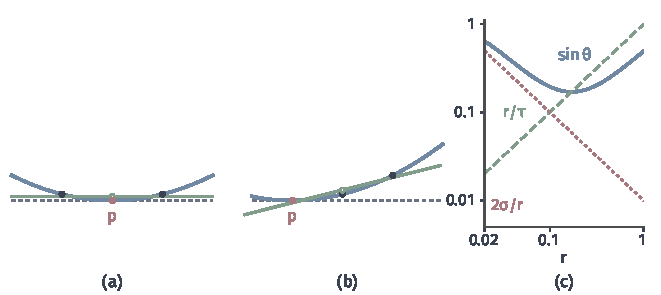
\includegraphics[width=112mm]{figures/04-spaces-measures-and-geometry/04-manifolds/matplotlib/mrec-pca/figure.pdf}
  \caption{局部PCA的方向误差。(a)(b) 抛物线$y=u^2/2$上$h=0.25$的对称与单侧邻域，黑点是样本，空心点是局部质心，绿线是主方向，虚线是$\bm{p}$处的真实切线；单侧时主方向倾斜$14.1^\circ$。(c) 单位圆上单侧弧$[0,r]$内$41$个样本加法向扰动$\sigma=0.005$时的实际误差（蓝），与弯曲项$r/\tau$（绿）、扰动项$2\sigma/r$（红）的比较，纵轴和横轴都取对数。}
  \label{fig:mrec-pca}
\end{BookInlineFigure}

\section{局部流形拟合}
\label{sec:mrec-local-fit}

切空间估计只给出一个平面，而流形在邻域内是弯的。要得到穿过或逼近样本的连续曲面片，还需要描述法向上怎样随切向坐标变化。本节在估计的平面上建立局部坐标，把法向分量拟合成切向坐标的函数，再分析拟合片的误差以及多片能否拼起来。拟合目标的加权、正则化等更一般的选择，以及相应的数值优化，属于\BookChapterRef{chap:optimization}{卷五第1章“优化问题与解”}开始的优化理论，本节只用普通最小二乘。

\subsection{局部图函数的拟合}
\label{sec:mrec-graph-fit}

设已选定局部中心$\bm q\in\mathbb R^D$，例如一个样本或局部质心，以及估计子空间的标准正交基$\widehat{\bm U}\in\mathbb R^{D\times m}$。把它补成$\mathbb R^D$的标准正交基$[\widehat{\bm U},\widehat{\bm V}]$，对邻域内每个观测计算切向坐标与法向分量
\[
 \bm u_j=\widehat{\bm U}^\top(\bm x_j-\bm q)\in\mathbb R^m,\qquad
 \bm w_j=\widehat{\bm V}^\top(\bm x_j-\bm q)\in\mathbb R^{D-m}.
\]
目标是找函数$g$使$\bm w_j\approx g(\bm u_j)$，由此得到连续片
\begin{equation}
 \bm\phi(\bm u)=\bm q+\widehat{\bm U}\bm u+\widehat{\bm V}g(\bm u),\qquad\bm u\in\Omega ,
 \label{eq:mrec-patch}
\end{equation}
其中$\Omega\subseteq\mathbb R^m$是切向坐标的定义域，例如半径为$\rho$的球。

\paragraph{图表示的前提}

只有当流形在这个邻域内确实是估计平面上的图时，拟合才有意义。把$M$上的点投影到估计平面，这个映射在$\bm p$处的导数是从$T_{\bm p}M$到$\widehat S$的正交投影，它的奇异值是两个子空间主夹角的余弦。只要最大主夹角小于$\pi/2$，导数就可逆，由反函数定理，$M$在$\bm p$附近可以写成$\bm q+\widehat{\bm U}\bm u+\widehat{\bm V}\widetilde g(\bm u)$，$\widetilde g$是$C^2$的。夹角越小、邻域越小，这个图表示的定义域越大、$\widetilde g$越平缓。

\paragraph{为什么要保留常数项和一次项}

真实切空间上的图函数满足$g(\bm0)=\bm0$与$Dg(\bm0)=\bm0$，但估计平面上的$\widetilde g$一般不满足：$\bm q$未必在$M$上，所以$\widetilde g(\bm0)\neq\bm0$；估计平面有倾斜，所以$D\widetilde g(\bm0)\neq\bm0$。在例~\ref{ex:mrec-one-sided}中，估计方向的斜率约为$h/R$，抛物线在新坐标下于$\bm p$处的斜率约为$-h/R$。若强行要求一次项为零，邻域边缘$|u|\approx2h$处的拟合误差就有$2h^2/R$量级，与弯曲本身一样大。

所以把估计平面的偏差纳入模型，用含常数项、一次项和二次项的多项式拟合每个法向分量：
\[
 g(\bm u)=\bm c_0+\bm L\bm u+\bigl(\tfrac12\bm u^\top\bm Q_l\bm u\bigr)_{l=1}^{D-m},
\]
其中$\bm c_0\in\mathbb R^{D-m}$，$\bm L\in\mathbb R^{(D-m)\times m}$，每个$\bm Q_l$是$m$阶对称矩阵。每个法向分量有$1+m+m(m+1)/2$个系数，$m=1$时为$3$个，$m=2$时为$6$个。

\paragraph{系数的求解与约束}

系数关于数据是线性的。把每个$\bm u_j$处全部单项式的值排成一行，得到设计矩阵$\bm\Phi\in\mathbb R^{k\times N_c}$，$N_c=1+m+m(m+1)/2$；每个法向分量的系数是以$\bm\Phi$为设计矩阵的普通最小二乘解，其构造与核对可参考\BookChapterRef{chap:linear-solution-selection}{卷二第9章“线性方程与最小二乘的选解”}。系数唯一当且仅当$\bm\Phi$满列秩。

$\bm\Phi$满列秩有直接的几何含义：$\bm\Phi\bm a=\bm0$意味着系数为$\bm a$的二次多项式在全部$\bm u_j$处为零，所以$\bm\Phi$满列秩当且仅当没有非零的二次多项式在全部切向坐标处同时为零。$m=1$时，这要求至少有三个不同的$u_j$；$m=2$时，要求至少六个点且它们不全落在同一条二次曲线上，例如全部落在一条直线上就不行。这正是第~\ref{sec:mrec-coverage}节方向分布条件在二阶拟合中的形式。

\begin{example}[圆弧上的二次拟合]
\label{ex:mrec-circle-fit}
在半径为$R$的圆的最低点取$\bm q=\bm p=(0,0)$，切线为横轴，样本取在横坐标$u=-h,0,h$处，纵坐标为$w=c,0,c$，$c=R-\sqrt{R^2-h^2}$。三点恰好确定二次多项式，解得$g(u)=(c/h^2)u^2$，常数项与一次项为零，这是对称性的结果。

二次系数$c/h^2=1/(R+\sqrt{R^2-h^2})$，当$h\to0$时趋于$1/(2R)$，与真实图函数$R-\sqrt{R^2-u^2}=u^2/(2R)+u^4/(8R^3)+\cdots$的二次项一致。在样本处拟合与真值相等，在其他位置的差别来自四次项，$|u|\leq h$时为$h^4/R^3$量级。
\end{example}

\subsection{局部片的误差与拼接}
\label{sec:mrec-patch-error}

拟合片要与真实流形比较，就要在同一个定义域上比较同一种量。在估计平面的坐标域$\Omega$上，真实流形写成$\widetilde g$，拟合片写成$g$，法向偏差是$\sup_{\bm u\in\Omega}\lVert g(\bm u)-\widetilde g(\bm u)\rVert_2$。这个量把以下几种误差合在了一起，分析时要分别检查。

\paragraph{误差的来源}

第一是切空间估计的偏差。它本身不是拟合误差，而是改变了$\widetilde g$的形状：倾斜越大，$\widetilde g$的一次项越大、图表示的定义域越小，夹角接近$\pi/2$时图表示不复存在。模型含一次项可以吸收小的倾斜，但不能挽救大的倾斜。

第二是函数截断。$\widetilde g$一般不是二次多项式。若它是$C^3$的，在半径为$\rho$的定义域上，二次Taylor多项式的余项为$\rho^3$量级；若只知道它是$C^2$的，则只能说余项比$\rho^2$小，没有确定的阶。截断误差指$\widetilde g$中任何二次多项式都消除不了的部分，Taylor余项给出它的一个上界；最小二乘所得的多项式不一定就是Taylor多项式，但它也不可能比最好的二次多项式更接近$\widetilde g$。

第三是样本分布与观测噪声。设法向数据是$\widetilde g(\bm u_j)$加上偏差$\bm\eta_j$，偏差中既有截断余项，也有观测扰动。最小二乘系数的误差不超过$\lVert\bm\eta\rVert_2/\sigma_{\min}(\bm\Phi)$，其中$\sigma_{\min}(\bm\Phi)$是设计矩阵的最小奇异值；切向坐标挤在一起或接近落在同一条二次曲线上时，$\sigma_{\min}$小，偏差被放大。有界扰动可以有系统的方向，增加样本数并不自动使它平均掉。

\paragraph{函数值误差不控制导数}

法向偏差小，不说明拟合片的切方向或曲率也准确。设真实流形在局部是$w=0$的直线，观测沿$u$方向以间距$s$交替带有$+\sigma$与$-\sigma$的法向扰动。若用插值样本的折线作拟合片，每一点的函数值误差不超过$\sigma$，斜率却到处是$\pm2\sigma/s$；$s$越小，即样本越密，斜率误差反而越大。

固定阶数的多项式不会这样振荡，但它与$\widetilde g$之差一般不是多项式，函数值上的误差界不能直接换成导数上的误差界。要从拟合片读出切方向或曲率，需要对导数单独分析误差，函数值逼近只是其中一个条件。

\paragraph{多片的并不自动是流形}

在每个样本附近各拟合一片以后，所有片的并未必是光滑流形。相邻两片在重叠区域可能不一致，留下台阶或缝隙；来自两个相近分支的片可能彼此穿过，并集出现自交，在交线附近根本不是流形。要拼成一个整体，至少需要相邻片的坐标域相互重叠、在重叠处的坐标转换光滑且一致，并用适当的方式把各片平滑地合成一张曲面。

即使拼接成功，所得曲面与真实流形同胚，也需要额外的条件和论证，这已超出本节的范围。后面的同调恢复不以局部拟合为前提：第~\ref{sec:mrec-homology-recovery}节直接由样本的球并与复形得到拓扑信息，不需要先构造曲面。

\section{内在距离逼近}
\label{sec:mrec-intrinsic-distance}

沿流形从一点走到另一点有多远，即内在距离$d_M$，不能由两点的环境距离读出：螺旋卷起的纸面上，相邻两层的点环境距离很小，沿纸面却要绕很远。但在很小的尺度上，环境距离与内在距离几乎相同。于是可以用短边连接相邻的样本，再沿图上的路径把短距离一段段累加起来，逼近远处两点之间的内在距离。本节只在同一连通分支内比较，不同分支之间的内在距离为无穷，图上相应的距离也应为无穷。

\subsection{邻接图的构造}
\label{sec:mrec-neighborhood-graph}

先讨论按固定半径连边的图，它对应一个明确的几何尺度。

\begin{definition}[半径邻域图与图距离]
\label{def:mrec-neighborhood-graph}
给定样本$P=\{\bm p_1,\ldots,\bm p_n\}$和半径$r>0$，\term{邻域图}（neighborhood graph）$\mathcal G_r$以样本为顶点，$\lVert\bm p_i-\bm p_j\rVert_2\leq r$时连边$\{i,j\}$，边权为$\lVert\bm p_i-\bm p_j\rVert_2$。顶点$i,j$之间的\term{图距离}（graph distance）$d_{\mathcal G}(i,j)$是连接它们的路径的边权和的最小值，没有路径时为$+\infty$。
\end{definition}

图距离可以用最短路算法计算，边权非负时Dijkstra算法适用，可参考\BookChapterRef{chap:shortest-paths}{卷三第3章“最短路”}。这里的输入只有样本之间的环境距离，与直接使用流形上的测地距离不同：边权是弦长，不是弧长，并且只有不超过$r$的弦才被使用。每条边的弦长都不超过两端点的内在距离，这是低估的来源；路径只能经过样本，不能走真实的最短曲线，这是高估的来源。下一小节说明两者怎样平衡。

\paragraph{其他连边规则}

另一种常用规则是近邻图：每个样本连向离它最近的$k$个样本。这个关系不对称，$\bm p_j$是$\bm p_i$的近邻，$\bm p_i$未必是$\bm p_j$的近邻，需要声明用“或”还是用“且”把它对称化。更重要的是，固定$k$并不固定几何尺度：稀疏处第$k$个近邻可能很远，稠密处则很近。

所以近邻图要按它实际产生的边来核对条件：最长的边是否小于可达半径给出的界，最短的那些边是否足以跨过采样的空隙。下面的结论只依赖“所有边都不超过某个长度”与“所有足够短的点对都连了边”这两条性质，对近邻图需要分别验证。

\paragraph{连通不等于可靠}

图是否连通与图距离是否可靠是两回事。一条错误地连接了两个远处部分的边，会使图更加连通，同时让大量点对的图距离严重偏小。反过来，图不连通时，同一分支内的点对会得到无穷的图距离，这也是错的。连通性只是一个必要的检查，不能代替下面的误差分析。

\subsection{图距离的误差}
\label{sec:mrec-graph-distance-error}

下面假定样本在$M$上、无噪声，用覆盖精度$\delta$与可达半径$\tau$控制图距离与内在距离之比。

\begin{theorem}[图距离逼近内在距离]
\label{thm:mrec-graph-distance}
设$P\subseteq M$，$M$上每一点到最近样本的环境距离不超过$\delta$，邻域图半径满足$2\delta<r<2\tau$。则$\mathcal G_r$的边只连接同一分支的样本；对同一分支中的任意两个样本$\bm p,\bm q$，
\[
 \frac{r/(2\tau)}{\arcsin\bigl(r/(2\tau)\bigr)}\,d_M(\bm p,\bm q)
 \leq d_{\mathcal G}(\bm p,\bm q)
 \leq\Bigl(1+\frac{2\delta}{r-2\delta}\Bigr)d_M(\bm p,\bm q).
\]
\end{theorem}
\begin{proof}
先证上界。记$\ell=r-2\delta>0$。任取$\varepsilon>0$和一条连接$\bm p,\bm q$、长度$L<d_M(\bm p,\bm q)+\varepsilon$的曲线$\gamma$，按弧长参数化。令$K=\lceil L/\ell\rceil$，$t_k=k\ell$（$k<K$），$t_K=L$。取$\bm s_0=\bm p$、$\bm s_K=\bm q$，其余$\bm s_k$取为离$\gamma(t_k)$不超过$\delta$的样本。

相邻两点的环境距离不超过它们之间的弧长，所以
\[
 \lVert\bm s_k-\bm s_{k+1}\rVert_2\leq\lVert\bm s_k-\gamma(t_k)\rVert_2+(t_{k+1}-t_k)+\lVert\gamma(t_{k+1})-\bm s_{k+1}\rVert_2\leq\delta+\ell+\delta=r,
\]
每一对相邻点之间都有边。把上式对$k$求和，两端的$\bm s_0,\bm s_K$与曲线上的点重合，只有$K-1$个中间点各贡献两次$\delta$，于是图上这条路径的长度不超过$L+2\delta(K-1)$。由$K-1<L/\ell$，
\[
 d_{\mathcal G}(\bm p,\bm q)\leq L\Bigl(1+\frac{2\delta}{\ell}\Bigr)<\bigl(d_M(\bm p,\bm q)+\varepsilon\bigr)\Bigl(1+\frac{2\delta}{r-2\delta}\Bigr),
\]
令$\varepsilon\to0$即得上界。

再证下界。每条边长$a\leq r<2\tau$，由定理~\ref{thm:mrec-reach-consequences}，两端属于同一分支，且其内在距离不超过$2\tau\arcsin(a/(2\tau))$。函数$x\mapsto\arcsin(x)/x$在$(0,1]$上递增，所以这又不超过$a\cdot\frac{2\tau}r\arcsin\frac r{2\tau}$。对图上任一条从$\bm p$到$\bm q$的路径，由$d_M$的三角不等式，$d_M(\bm p,\bm q)$不超过各边内在距离之和，从而不超过路径长度乘以$\frac{2\tau}r\arcsin\frac r{2\tau}$。对全部路径取最小即得下界。
\end{proof}

两个比例因子分别说明误差从哪里来。下界的因子只依赖$r/\tau$：边越短、流形越不弯，弦与弧越接近，例如$r=\tau/2$时因子为$0.25/\arcsin0.25\approx0.989$。上界的因子只依赖$\delta/r$：样本越密，路径越不必绕行，例如$\delta=r/10$时因子为$1.25$。两者同时趋于$1$，需要$\delta\ll r\ll\tau$，与第~\ref{sec:mrec-neighborhood-scale}节的尺度要求一致。

\paragraph{两类失效}

条件不满足时，误差可以任意大，而且方向相反。第一类是缺采样。在单位圆上，若某段圆心角为$\alpha$的弧内没有样本，而弦长$2\sin(\alpha/2)$大于$r$，跨越空缺的边就不存在，空缺两端的样本只能绕另一侧相连，图距离约为$2\pi-\alpha$，而真实内在距离只有$\alpha$。若圆上有两处这样的空缺，图会断成两段，同一分支内的点对得到无穷的图距离。这违反了定理中的覆盖条件$2\delta<r$。

第二类是邻接过大。若一条闭曲线折成发卡形，两股相距$2b$，而$r\geq2b$，两股之间就会连上边，原本沿曲线相距很远的两点，图距离只有约$2b$。这时$\tau\leq b$，所以$r\geq2\tau$，违反了定理中的另一个条件。两类失效分别对应上界和下界的条件，一个让图距离过大，一个让它过小。

\paragraph{离开流形的噪声}

观测带有扰动$\lVert\bm x_i-\bm p_i\rVert_2\leq\sigma$时，邻域图按观测之间的距离$\lVert\bm x_i-\bm x_j\rVert_2$构造，定理的条件需要重新建立。由三角不等式，每条边两端真实位置的距离不超过边长加$2\sigma$，所以要保证不跨接分支，应要求$r+2\sigma<2\tau$；而边长本身与真实弦长之差可达$2\sigma$。

一条有$K$条边的路径，累积的边长误差可达$2\sigma K$。沿长度为$L$的曲线，所需边数约为$L/r$，于是相对误差约为$2\sigma/r$。所以噪声要求$\sigma\ll r$，并且覆盖条件要用观测的覆盖精度，即真实覆盖精度加上$\sigma$。这些是新增的条件，无噪声情形的定理不能直接沿用。


\section{同调恢复}
\label{sec:mrec-homology-recovery}

前几节恢复的都是局部的量。流形有几个分支、有几个洞，是整体的拓扑信息，单看任何一个邻域都无法知道。第~\ref{chap:homology}章用同调空间的维数，即Betti数，记录这类信息：$\beta_0$是连通分支数，圆的$\beta_1=1$对应绕一圈的环。本节研究怎样只用有限样本算出底层流形的同调。

路线分三步。先把离散的样本加粗成连续的空间，即以样本为球心的球并；再用有限的组合数据记录球与球怎样交叠，得到Čech复形与Rips复形；最后用神经引理和形变收缩证明，在适当的尺度下，复形的同调等于流形的同调。整个论证得到的是同伦等价与同调同构，不是同胚，更不是光滑结构的恢复。

\subsection{样本的球并}
\label{sec:mrec-ball-union}

有限点集的拓扑是平凡的：每个点自成一个分支，没有任何洞。要让样本“连成一片”，最直接的办法是把每个样本加粗成一个小球。给定样本$P$与半径$r>0$，记
\begin{equation}
 U_r=\bigcup_{\bm p\in P}B(\bm p,r),
 \label{eq:mrec-ball-union}
\end{equation}
其中$B(\bm p,r)$是环境空间中的开球。\term{球并}（union of balls）$U_r$是$\mathbb R^D$的开集，它的拓扑随$r$变化。

以单位圆上正六边形的六个顶点为样本，相邻顶点相距$1$，图~\ref{fig:mrec-hexagon}第一行画了三种半径。$r\leq\tfrac12$时六个球互不相交，$U_r$有六个分支。$\tfrac12<r\leq1$时相邻的球交叠，球并连成一个环；圆心到各样本的距离为$1$，不在任何开球中，绕圆心的洞还在。$r>1$时每个球都含圆心，球并关于圆心是星形的，可以沿直线收缩到圆心，洞被填掉了。

这个例子说明覆盖条件的作用和局限。若$M$上每一点到最近样本的距离小于$\delta$，则$r\geq\delta$时$M\subseteq U_r$。但包含不等于保持拓扑：上例$r>1$时球并包含圆，却已没有洞。球并在什么半径下与$M$有相同的拓扑，要结合第~\ref{sec:mrec-reach}节的可达半径判断，这是第~\ref{sec:mrec-recovery-scale}节的问题。

\begin{BookInlineFigure}
  \centering
  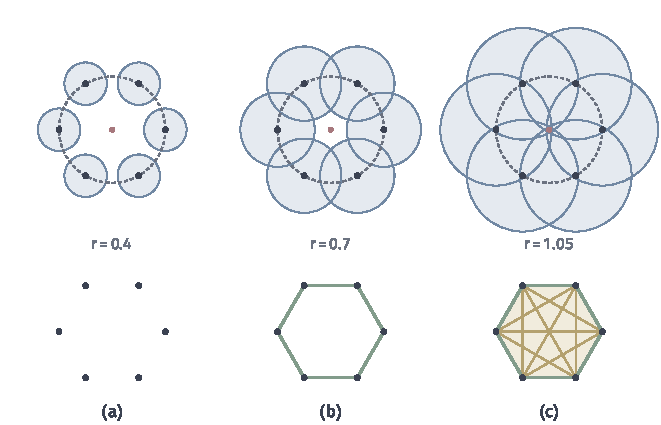
\includegraphics[width=112mm]{figures/04-spaces-measures-and-geometry/04-manifolds/matplotlib/mrec-hexagon/figure.pdf}
  \caption{单位圆上正六边形样本的球并（第一行）与对应的Čech复形（第二行）。虚线是单位圆，红点是圆心。(a) 六个球互不相交，复形只有六个顶点。(b) 相邻的球交叠成环，圆心未被覆盖，复形是六边形的边界。(c) 每个球都含圆心，复形的所有子集都是单纯形（浅黄表示填充），洞消失。}
  \label{fig:mrec-hexagon}
\end{BookInlineFigure}

\subsection{Čech复形}
\label{sec:mrec-cech}

球并是连续空间，不能直接放进计算机。它的拓扑由球与球怎样交叠决定，而交叠关系是有限的组合数据：哪些球两两相交，哪些三个球有公共点，等等。

\begin{definition}[Čech复形]
\label{def:mrec-cech}
给定欧氏空间中的有限点集$P$与半径$r>0$，\term{Čech复形}（Čech complex）$\check C_r(P)$由所有满足$\bigcap_{\bm p\in\sigma}B(\bm p,r)\neq\varnothing$的非空子集$\sigma\subseteq P$组成，其中$B(\bm p,r)$是开球。
\end{definition}

若一组球有公共点，其中任意几个球也有，所以$\check C_r(P)$对取子集封闭，是第~\ref{chap:homology}章意义下的抽象单纯复形。条件$\bigcap_{\bm p\in\sigma}B(\bm p,r)\neq\varnothing$等价于存在一点到$\sigma$中每个点的距离都小于$r$，即覆盖$\sigma$的最小闭球半径小于$r$。特别地，两点连边当且仅当它们的距离小于$2r$。

Čech复形记录的是整个球族的交叠，不只是两两的交叠。取边长为$0.9$的正三角形，$r=0.5$，如图~\ref{fig:mrec-cech-rips}。三对球两两相交，因为$0.9<1$；但覆盖三个顶点的最小球是外接球，半径
\[
 \frac{0.9}{\sqrt3}\approx0.520>0.5,
\]
三个球没有公共点。所以$\check C_{0.5}$只有三条边，没有三角形，留下一个一维的环；$r$增大到超过$0.520$时三角形被填上，环随之消失。$r\leq r'$时$\check C_r\subseteq\check C_{r'}$，尺度变化改变的正是这种填充关系。

回到正六边形，把顶点依次编号为$0,\ldots,5$。$\tfrac12<r\leq\tfrac{\sqrt3}2$时复形是六边形的边界。$r$超过$\tfrac{\sqrt3}2$后，隔一个顶点的两点连边，三个相邻顶点组成的三角形也被填上，但这些三角形都贴着外圈，中间的洞还在；直到$r>1$时，含对径点的单纯形和三角形$\{0,2,4\}$、$\{1,3,5\}$才出现，把洞填上。复形的同调与球并的同调随$r$同步变化，这不是巧合，第~\ref{sec:mrec-nerve-lemma}节解释原因。

\subsection{Rips复形}
\label{sec:mrec-rips}

判断三个以上的球有没有公共点，需要计算最小覆盖球，在高维中代价不小，而且要用到点的坐标。只用成对距离的替代方案是Rips复形。

\begin{definition}[Rips复形]
\label{def:mrec-rips}
给定有限点集$P$与它们之间的距离，以及$r>0$，\term{Rips复形}（Vietoris--Rips complex）$R_r(P)$由所有直径不超过$r$的非空子集$\sigma\subseteq P$组成，即$\sigma$中任意两点的距离都不超过$r$。
\end{definition}

判定一个单纯形只需要它各顶点之间的成对距离，所以Rips复形可以直接由距离表构造，不需要坐标，也不需要距离来自欧氏点。它由边完全确定：一组顶点构成单纯形，当且仅当其中两两之间都有边。这既是计算上的便利，也意味着它丢失了“成对相交而无公共点”的区别。

\begin{BookInlineFigure}
  \centering
  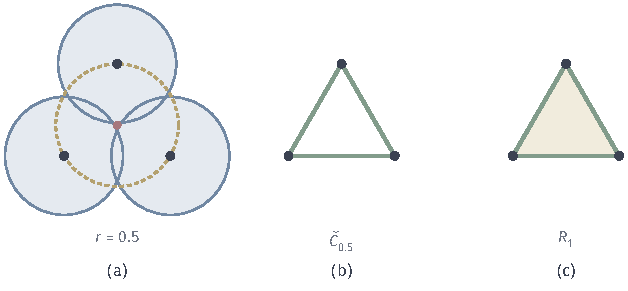
\includegraphics[width=106.299mm]{figures/04-spaces-measures-and-geometry/04-manifolds/tikz/mrec-cech-rips/figure.pdf}
  \caption{边长$0.9$的正三角形。(a) 半径$0.5$的三个球两两相交，但没有公共点；虚线是半径约$0.520$的外接圆，圆心（红）在三个开球之外。(b) Čech复形$\check C_{0.5}$只有三条边，中间是空的。(c) Rips复形$R_1$只看成对距离，三边都不超过$1$，三角形被填上。}
  \label{fig:mrec-cech-rips}
\end{BookInlineFigure}

比较两种复形时，要注意参数的含义不同：Čech复形的$r$是开球半径，Rips复形的$r$是闭的直径界。在上例中，$R_1$含有那个三角形，$\check C_{0.5}$不含，二者连边的条件几乎相同，却不是同一个复形。两者之间有如下的夹逼关系：对任意$\eta>0$，
\begin{equation}
 \check C_r(P)\subseteq R_{2r}(P)\subseteq\check C_{2r+\eta}(P).
 \label{eq:mrec-cech-rips}
\end{equation}

第一个包含：若$\sigma$中各点到某个$\bm z$的距离都小于$r$，则任意两点距离小于$2r$。第二个包含：若$\sigma$的直径不超过$2r$，取$\sigma$中任一顶点作为公共点，它到其余顶点的距离不超过$2r<2r+\eta$。这些常数足以使用，但不是最紧的。夹逼关系说明两种复形在尺度相差一倍的范围内相互控制，不能在同一个数值参数下直接等同。

\subsection{神经引理}
\label{sec:mrec-nerve-lemma}

Čech复形是球并的组合记录，现在要说明这一记录没有丢失同伦信息。一般地，给定一族集合，可以只记录哪些成员有公共点。

\begin{definition}[神经与良覆盖]
\label{def:mrec-nerve}
设$\mathcal U=\{U_1,\ldots,U_n\}$是一族集合。它的\term{神经}（nerve）$N(\mathcal U)$是以$\{1,\ldots,n\}$为顶点集的抽象单纯复形，非空子集$\sigma$是单纯形当且仅当$\bigcap_{i\in\sigma}U_i\neq\varnothing$。若每个非空的有限交$\bigcap_{i\in\sigma}U_i$都是可缩空间，则称$\mathcal U$为\term{良覆盖}（good cover），这里覆盖指它覆盖并集$\bigcup_iU_i$。
\end{definition}

按定义，$\check C_r(P)$就是开球族$\{B(\bm p,r)\}_{\bm p\in P}$的神经。有限个欧氏开球构成良覆盖：凸集的交仍是凸集，非空凸集$K$可以沿直线收缩到其中一点$\bm z_0$，同伦取
\[
 H(\bm x,t)=(1-t)\bm x+t\bm z_0 ,
\]
凸性保证$H(\bm x,t)\in K$，所以$K$可缩。

\begin{theorem}[神经引理]
\label{thm:mrec-nerve-lemma}
设$\mathcal U$是$\mathbb R^D$中有限个开凸集组成的族，则神经的几何实现$\lvert N(\mathcal U)\rvert$与并集$\bigcup_iU_i$同伦等价。特别地，对有限点集$P$和任意$r>0$，$\lvert\check C_r(P)\rvert$与球并$U_r$同伦等价。
\end{theorem}

完整的证明较长，读者可查阅Hatcher《代数拓扑》中关于神经的推论。这里构造两个方向的映射，并验证其中一个复合同伦于恒等映射，这已经能看出凸性起的作用。

从并集到神经：取一组连续函数$\varphi_i\geq0$，在$U_i$内为正、在$U_i$外为零，且处处$\sum_i\varphi_i=1$，例如把$\bm x$到$U_i$补集的距离归一化。令$F(\bm x)=\sum_i\varphi_i(\bm x)\bm v_i$，$\bm v_i$是第$i$个顶点。$\varphi_i(\bm x)>0$的那些$i$对应的集合都含$\bm x$，有公共点，所以$F(\bm x)$落在神经中的一个单纯形内。

反方向，在每个非空交$\bigcap_{i\in\sigma}U_i$中取一点$\bm c_\sigma$，在$\lvert N(\mathcal U)\rvert$的重心细分上，把$\sigma$的重心送到$\bm c_\sigma$，再在细分的每个单纯形上线性延拓，得到$G$。细分中的单纯形对应一串$\sigma_0\subseteq\cdots\subseteq\sigma_k$，所有$\bm c_{\sigma_j}$都在凸集$\bigcap_{i\in\sigma_0}U_i$中，所以$G$的像落在并集内。

现在看$G\circ F\simeq\mathrm{id}$。设$F(\bm x)$落在细分单纯形$\sigma_0\subseteq\cdots\subseteq\sigma_k$内，此时$\sigma_k$中的每个集合都含$\bm x$，特别是$\sigma_0$中的每个集合都含$\bm x$。于是$\bm x$与$G(F(\bm x))$都在凸集$\bigcap_{i\in\sigma_0}U_i$中，连接它们的线段也在其中，直线同伦$(1-t)\bm x+tG(F(\bm x))$就留在并集内。

另一个复合$F\circ G$同伦于恒等映射，这一步要复杂得多，需要在神经上逐层构造同伦，完整的论证见上面所指的文献。

神经引理把连续空间的问题转为有限计算。由第~\ref{chap:homology}章的同伦不变性，同伦等价的空间有同构的同调，几何实现的同调又等于单纯同调，于是
\begin{equation}
 H_k(U_r)\cong H_k\bigl(\lvert\check C_r(P)\rvert\bigr)\cong H_k\bigl(\check C_r(P)\bigr),
 \label{eq:mrec-nerve-homology}
\end{equation}
右端只需写出$\check C_r(P)$的边界矩阵并计算秩。正六边形的例子正是这样：$\tfrac12<r\leq\tfrac{\sqrt3}2$时，复形是六个顶点、六条边的环，边界矩阵的秩为$5$，$\beta_1=6-5=1$，与球并的环对应。

\subsection{恢复尺度}
\label{sec:mrec-recovery-scale}

至此，球并的同调可以由Čech复形算出。剩下的问题是：球并的同调何时等于$M$的同调？回到第~\ref{sec:mrec-ball-union}节的六边形，半径太小时球并断开，太大时洞被填掉，需要一个既不太小也不太大的半径。

\paragraph{两类条件}

第一类条件是覆盖：$M\subseteq U_r$，否则流形上未被覆盖的部分会让球并断开或多出洞。若样本是$\delta$稠密的，$r\geq\delta$即可。

第二类条件是不错误地连接或填充：球并不能把流形相距较远的部分接起来，也不能把流形围出的洞盖住。由于球心都在$M$上，$U_r$中每一点到$M$的距离小于$r$；若$r<\tau$，$U_r\subseteq M^\tau$，最近点投影$\pi$在整个$U_r$上有定义。

两类条件写成同一个半径的允许范围：$r$要大于某个由覆盖精度决定的下界，又要小于某个由可达半径决定的上界。只有覆盖精度相对可达半径足够小时，这个范围才非空。只看样本很密，或只看球并连通，都推不出恢复：六边形样本在$r=1.01$时球并连通且包含圆，同调却已与圆不同。

\paragraph{形变收缩的前提}

要证明$U_r$与$M$有同样的同调，最自然的方法是把$U_r$形变收缩到$M$上：令
\begin{equation}
 F(\bm x,t)=(1-t)\bm x+t\,\pi(\bm x),
 \label{eq:mrec-retraction}
\end{equation}
把每一点沿直线推向它的最近点，如图~\ref{fig:mrec-retraction}(a)。$t=0$时是恒等映射，$t=1$时落在$M$上，$M$上的点始终不动。第~\ref{chap:homology}章说明形变收缩是同伦等价。

这一构造需要两个前提。一是$\pi$在$U_r$上有定义且连续，由$r<\tau$保证。二是从$\bm x$到$\pi(\bm x)$的线段整个留在$U_r$中，否则$F$会离开$U_r$，不是$U_r$上的形变。第二个前提并不平凡：线段从$\bm x$所在的球出发，它的另一端$\pi(\bm x)$可能落在别的球里，中间不能经过球并之外的缝隙。下一小节的证明处理的就是这件事。

\paragraph{圆上的核对}

单位圆的可达半径为$\tau=1$。下一小节的定理要求样本是$\varepsilon/2$稠密的，且$\varepsilon<\sqrt{3/5}\,\tau\approx0.775$，所以覆盖精度必须小于约$0.387$。

正六边形的覆盖精度是$0.518$，不满足条件。尽管如此，$r=0.6$时球并覆盖了圆，又没有盖住圆心，同调仍然正确；定理的条件是充分的，不是必要的。

改取$24$个等距样本，覆盖精度为$0.131$。允许的半径范围是$2\times0.131<\varepsilon<0.775$，例如$\varepsilon=0.3$，图~\ref{fig:mrec-retraction}(a)画的就是这个球并。在这个范围内，定理保证球并的同调等于圆的同调，即$\beta_0=\beta_1=1$。

\subsection{同调恢复定理}
\label{sec:mrec-homology-theorem}

把上面的条件定量化，就得到Niyogi、Smale与Weinberger的结果。

\begin{theorem}[有限样本的同调恢复]
\label{thm:mrec-homology-recovery}
设$M\subseteq\mathbb R^D$是紧致无边界的光滑嵌入子流形，可达半径为$\tau>0$。设有限样本$P\subseteq M$是$\varepsilon/2$稠密的，即$M$上每一点到最近样本的环境距离小于$\varepsilon/2$，且$0<\varepsilon<\sqrt{3/5}\,\tau$。则式~\eqref{eq:mrec-ball-union}的球并$U_\varepsilon$形变收缩到$M$，从而对每个$k$，
\begin{equation}
 H_k(M)\cong H_k(U_\varepsilon)\cong H_k\bigl(\check C_\varepsilon(P)\bigr).
 \label{eq:mrec-homology-recovery}
\end{equation}
\end{theorem}

证明的关键是说明线段$[\bm x,\pi(\bm x)]$留在球并中。思路是分两种情形：要么$\pi(\bm x)$就在$\bm x$所在的球内，线段自然留在这个凸的球里；要么$\pi(\bm x)$离球心较远，这时可以证明$\bm x$离流形很近，于是整条线段都落在$\pi(\bm x)$附近某个样本的球里，如图~\ref{fig:mrec-retraction}(b)。

\begin{proof}
由$\varepsilon/2$稠密，$M\subseteq U_\varepsilon$。由$\varepsilon<\tau$，$U_\varepsilon\subseteq M^\tau$，$\pi$在$U_\varepsilon$上连续。下面证明对任一$\bm x\in U_\varepsilon$，线段$[\bm x,\pi(\bm x)]$留在$U_\varepsilon$中。

设$\bm x\in B(\bm p,\varepsilon)$，$\bm p\in P$。记$\bm q=\pi(\bm x)$，并记
\[
 T=\lVert\bm x-\bm q\rVert_2,\qquad a=\lVert\bm p-\bm q\rVert_2 .
\]
$T=0$时无需证明。否则令$\bm v=(\bm x-\bm q)/T$，由一阶条件它是$\bm q$处的单位法向量。$\bm q$是最近点，所以
\[
 T\leq\lVert\bm x-\bm p\rVert_2<\varepsilon<\tau .
\]

情形一，$a<\varepsilon$。此时$\bm x,\bm q$都在开球$B(\bm p,\varepsilon)$中，球是凸的，线段留在其中。

情形二，$a\geq\varepsilon$。先估计$T$。由$\bm x-\bm p=(\bm q-\bm p)+T\bm v$，
\[
 \lVert\bm x-\bm p\rVert_2^2=a^2+T^2-2T\langle\bm p-\bm q,\bm v\rangle .
\]
由式~\eqref{eq:mrec-reach-normal}，$\langle\bm p-\bm q,\bm v\rangle\leq a^2/(2\tau)$，代入并用$\lVert\bm x-\bm p\rVert_2<\varepsilon$，得
\[
 \varepsilon^2>a^2\Bigl(1-\frac T\tau\Bigr)+T^2 .
\]
因为$T<\tau$，右端对$a$递增，代入$a\geq\varepsilon$，得$\varepsilon^2>\varepsilon^2(1-T/\tau)+T^2$，整理后
\begin{equation}
 T<\frac{\varepsilon^2}\tau .
 \label{eq:mrec-t-bound}
\end{equation}

再取样本$\bm q'$使$b=\lVert\bm q-\bm q'\rVert_2<\varepsilon/2$，这由稠密性保证。线段上的点可写成$\bm y=\bm q+t\bm v$，$0\leq t\leq T$。展开$\lVert\bm y-\bm q'\rVert_2^2$，并对$\bm q'-\bm q$的法向分量用式~\eqref{eq:mrec-reach-normal}，得
\[
 \lVert\bm y-\bm q'\rVert_2^2\leq b^2+t^2+\frac{tb^2}\tau .
\]
代入$b^2<\varepsilon^2/4$和式~\eqref{eq:mrec-t-bound}，
\[
 \lVert\bm y-\bm q'\rVert_2^2<\frac{\varepsilon^2}4+\frac{\varepsilon^4}{\tau^2}+\frac{\varepsilon^4}{4\tau^2}=\frac{\varepsilon^2}4+\frac54\cdot\frac{\varepsilon^4}{\tau^2}.
\]
由$\varepsilon^2<\tfrac35\tau^2$，第二项小于$\tfrac34\varepsilon^2$，于是$\lVert\bm y-\bm q'\rVert_2<\varepsilon$。整条线段都在球$B(\bm q',\varepsilon)$中。

这样，式~\eqref{eq:mrec-retraction}定义的$F$就是$U_\varepsilon$到$M$的形变收缩：它连续，$t=0$时是恒等映射，$t=1$时映入$M$，且保持$M$上的点不动。所以$M\hookrightarrow U_\varepsilon$是同伦等价，第一个同构成立。第二个同构是式~\eqref{eq:mrec-nerve-homology}。
\end{proof}

常数$\sqrt{3/5}$的来源就在这个证明里：它恰好使$\tfrac14+\tfrac54(\varepsilon/\tau)^2<1$。右端是有限复形的单纯同调，可以由边界矩阵的秩算出，这就是“由有限样本恢复同调”的含义。

\begin{BookInlineFigure}
  \centering
  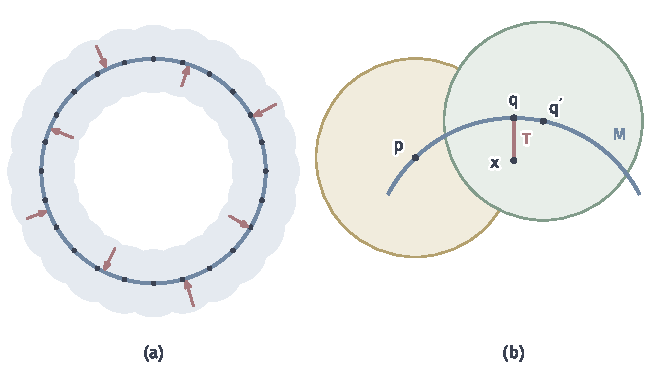
\includegraphics[width=112mm]{figures/04-spaces-measures-and-geometry/04-manifolds/matplotlib/mrec-retraction/figure.pdf}
  \caption{球并向流形的形变收缩。(a) 单位圆上$24$个等距样本、$\varepsilon=0.3$的球并（浅蓝），红色箭头把点沿线段推向最近点。(b) 证明情形二的几何（$\tau=1$，$\varepsilon=0.7$）：$\bm x$在$\bm p$的球（浅黄）中，但最近点$\bm q$不在其中；此时$T<\varepsilon^2/\tau$，线段$[\bm x,\bm q]$整条落在靠近$\bm q$的样本$\bm q'$的球（浅绿）中。}
  \label{fig:mrec-retraction}
\end{BookInlineFigure}

\paragraph{恢复的是什么}

定理恢复的是同调，而且是经由同伦等价得到的。它不给出与$M$同胚的空间：$U_\varepsilon$是$\mathbb R^D$中的开集，维数是$D$而不是$m$，与$M$同伦等价却不同胚；$\check C_\varepsilon(P)$可以含有维数远高于$m$的单纯形。至于$M$的光滑结构、度量或嵌入方式，定理没有给出任何信息。

定理的条件也划定了它的适用范围。样本必须在$M$上：观测离开流形时，需要把扰动界与覆盖精度、可达半径一起放进新的条件，并重新证明形变收缩。定理用的是Čech复形：改用Rips复形时，只能借助式~\eqref{eq:mrec-cech-rips}，在相差一倍的两个尺度之间比较，需要另行论证。从同调进一步恢复同胚类型，则需要完全不同的工具。

\section{持久同调}
\label{sec:mrec-persistence}

同调恢复定理要求半径落在一个由覆盖精度和可达半径决定的范围内，而这两个量通常并不知道，实际中只能尝试许多半径。逐个半径地报告Betti数会丢掉一个重要的信息：某个尺度下的一个环，与稍大尺度下的一个环，是不是同一个环。

可以把这件事想象成涨潮时看海岸：每个时刻拍一张照片，只数岛屿的个数，并不知道这个时刻的岛屿和下一时刻的岛屿谁是谁；若把录像连起来看，就能说清楚每个岛何时露出、何时被淹。本节让复形随尺度嵌套增长，用包含诱导的线性映射追踪同调类，得到的表示称为\term{持久同调}（persistent homology）。随后研究这一表示对距离扰动的稳定性，并说明它与第~\ref{sec:mrec-homology-recovery}节的恢复保证是两回事。

\subsection{过滤与诱导映射}
\label{sec:mrec-filtration}

Čech复形与Rips复形都随尺度单调增长：$r\leq r'$时$\check C_r(P)\subseteq\check C_{r'}(P)$，$R_r(P)\subseteq R_{r'}(P)$。

\begin{definition}[过滤]
\label{def:mrec-filtration}
一族以实数$r\geq0$为指标的单纯复形$\{K_r\}$，若$r\leq r'$时$K_r$是$K_{r'}$的子复形，则称为一个\term{过滤}（filtration）。
\end{definition}

对有限点集，Rips过滤只在有限个尺度上发生变化，这些尺度是成对距离的取值；Čech过滤的变化尺度是各子集最小覆盖球的半径，也只有有限个。两个相邻变化尺度之间，复形保持不变。

对每个$r\leq r'$，包含$K_r\hookrightarrow K_{r'}$诱导线性映射
\begin{equation}
 f_{r,r'}:H_k(K_r)\to H_k(K_{r'}),
 \label{eq:mrec-induced-map}
\end{equation}
这里同调取实系数。第~\ref{chap:homology}章说明，恒等包含诱导恒等映射，两次包含的复合诱导映射的复合，所以$f_{r,r}$是恒等映射，并且$f_{r',r''}\circ f_{r,r'}=f_{r,r''}$。这一族线性空间与线性映射称为一个\term{持久模}（persistence module）。

\paragraph{过滤的例子}

取边长为$1$的正方形的四个顶点作Rips过滤，如图~\ref{fig:mrec-filtration}(a)。$r<1$时只有四个点，$\beta_0=4$。$1\leq r<\sqrt2$时四条边出现，组成一个四边形，$\beta_0=1$，$\beta_1=1$。$r\geq\sqrt2$时两条对角线出现，四个三角形和整个四面体随之加入，复形可缩，$\beta_0=1$，$\beta_1=0$。

再取数轴上的三个点$0$、$1$、$3$。$r<1$时有三个分支；$r=1$时点$0$与点$1$合并；$r=2$时点$1$与点$3$相连，只剩一个分支。映射$f_{0.5,1.5}$把点$0$与点$1$的类送到同一个类，把点$3$的类送到它自己。诱导映射记录了是哪两个分支合并，这是Betti数序列$3,2,1$所没有的。

\paragraph{Betti数不足以描述跨尺度信息}

下面两个过滤的一维Betti数在每个尺度上都相同，诱导映射却不同。这两个过滤是直接写出的抽象过滤，不必来自点集。

过滤甲：四边形$abcd$在$r=1$时出现，在$r=3$时加入一条对角线和两个三角形被填满。过滤乙：四边形$abcd$同样在$r=1$时出现，但在$r=2$时被填满，同时另一个四边形$efgh$在$r=2$出现，在$r=3$时被填满。两者的零维同调不同，下面只比较一维同调。

两者的$\beta_1$都是：$r<1$时为$0$，$1\leq r<3$时为$1$，之后为$0$。但在过滤甲中，$f_{1.5,2.5}$把$r=1.5$处的环送到$r=2.5$处的同一个环，是同构；在过滤乙中，$r=1.5$处的环在$r=2$时已被填满，$f_{1.5,2.5}=0$，$r=2.5$处的环是新出现的。只看每个尺度的Betti数，无法区分“一个环持续存在”与“一个环消失、另一个环出现”。

\begin{BookInlineFigure}
  \centering
  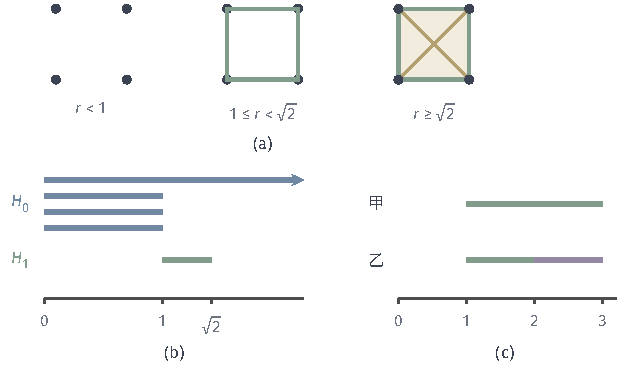
\includegraphics[width=105.346mm]{figures/04-spaces-measures-and-geometry/04-manifolds/tikz/mrec-filtration/figure.pdf}
  \caption{过滤与条形码。(a) 单位正方形的Rips过滤的三个阶段，浅黄表示填充的单纯形。(b) 正方形的条形码，蓝条是$H_0$（一根永不消失），绿条是$H_1$。(c) 过滤甲与过滤乙的$H_1$：逐尺度的Betti数相同，甲是一根贯穿的条，乙是前后相接的两根（绿、紫）。}
  \label{fig:mrec-filtration}
\end{BookInlineFigure}

\subsection{区间分解}
\label{sec:mrec-interval-decomposition}

持久模看起来是一串空间和映射，结构复杂。对有限点产生的过滤，它其实可以完全拆成最简单的块，每一块描述一个同调类从出现到消失的区间。

\paragraph{区间模与分解定理}

固定同调次数$k$。设$b<d\leq+\infty$，\term{区间模}（interval module）$I[b,d)$在$r\in[b,d)$处取$\mathbb R$，其余处取零空间；当$r\leq r'$都在$[b,d)$中时，映射是恒等映射，其余映射为零。它描述的正是一个在尺度$b$出现、在尺度$d$消失的同调类。

\begin{theorem}[区间分解]
\label{thm:mrec-interval-decomposition}
设过滤$\{K_r\}$由有限个复形组成，只在有限个尺度上变化，每个$K_r$都是有限复形。则对每个$k$，持久模$\{H_k(K_r),f_{r,r'}\}$同构于有限个区间模的直和$\bigoplus_lI[b_l,d_l)$，并且区间的多重集合$\{[b_l,d_l)\}$由持久模唯一确定。
\end{theorem}

证明要在所有尺度上同时选取相容的基，用到有限维空间中两个子空间族存在公共基的引理，篇幅较长，读者可查阅Zomorodian与Carlsson关于持久同调计算的论文。

结论的含义可以这样理解。可以在所有尺度上选取相容的基，使每个诱导映射都把基向量送到基向量或零。一个基向量对应一个区间，它出现的尺度是左端点，被送到零的尺度是右端点。这就像把线性映射化成对角形，只不过这里是一整串映射同时化简。两个分支合并时，约定保留出现较早的那个，较晚的那个记为消失，这一约定保证了分解的一致性。

由分解立刻得到一个常用的计数：$r\leq r'$时，$f_{r,r'}$的秩等于同时包含$r$和$r'$的区间的个数。

\paragraph{条形码与持久图}

区间的多重集合称为\term{条形码}（barcode），每个区间画成一根横条。也可以把每个区间$[b,d)$画成平面上的点$(b,d)$，分别称为出生坐标与死亡坐标，得到\term{持久图}（persistence diagram）；所有点都在对角线$b=d$上方，$d=+\infty$的点画在顶端。

端点的约定要说清。Rips过滤用闭条件，区间取左闭右开：类在尺度$b$已经存在，在尺度$d$恰好变为零或并入更早的类。Čech过滤用开球，单纯形在$r$严格超过阈值时才出现，区间实际是左开右闭的$(b,d]$，这只影响端点本身，不影响区间的长度和配对。不会在有限尺度消失的类对应$d=+\infty$，要保留在图中。

上一小节的例子可以直接读出条形码。正方形：$H_0$为$[0,\infty)$与三个$[0,1)$，$H_1$为$[1,\sqrt2)$。数轴上的三点：$H_0$为$[0,\infty)$、$[0,1)$、$[0,2)$。过滤甲的$H_1$为$[1,3)$，过滤乙的$H_1$为$[1,2)$与$[2,3)$，两者的区别清楚地显示出来，如图~\ref{fig:mrec-filtration}(b)(c)。

正六边形给出一个更有启发的比较。Rips过滤在$r=1$时出现六边形的环；$r=\sqrt3$时加入隔一个顶点的边，八个三角形恰好围成八面体的表面，环被填上，同时出现一个二维的空腔；$r=2$时加入对径的边，复形成为实心单纯形，空腔消失。所以$H_1$为$[1,\sqrt3)$，$H_2$为$[\sqrt3,2)$，见图~\ref{fig:mrec-barcodes}(a)。

Čech过滤的情形不同。由神经引理，它与平面中的球并同伦等价，而平面开集没有二维同调，所以没有$H_2$的条，$H_1$只有$(\tfrac12,1]$，见图~\ref{fig:mrec-barcodes}(b)。Rips过滤多出来的那根$H_2$条，正是它“成对相交就算有公共点”造成的，并不反映任何真实的二维结构。

条形码是跨尺度同调的表示，它不记录点的坐标，也不记录同胚类型或光滑结构。两组完全不同的点可以有相同的条形码，例如把整组点作任意合同变换，Rips过滤不变。

\begin{BookInlineFigure}
  \centering
  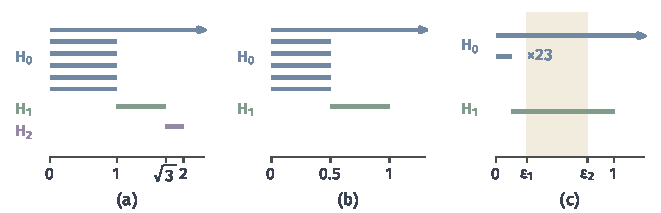
\includegraphics[width=112mm]{figures/04-spaces-measures-and-geometry/04-manifolds/matplotlib/mrec-barcodes/figure.pdf}
  \caption{由边界矩阵算出的条形码，横轴为尺度。(a) 单位正六边形的Rips过滤，$H_2$的条是八面体空腔。(b) 同一组点的Čech过滤，横轴为球半径，没有$H_2$。(c) 单位圆上$24$个等距样本的Čech过滤，$H_0$有$23$根相同的短条，$H_1$的唯一长条横跨浅黄色的恢复窗口$(\varepsilon_1,\varepsilon_2)$。}
  \label{fig:mrec-barcodes}
\end{BookInlineFigure}

\subsection{瓶颈距离}
\label{sec:mrec-bottleneck}

要谈条形码的稳定性，先要能比较两张持久图。数据稍有变化，长条的端点应该稍有移动，同时可能冒出或消失一些很短的条。比较时应把长条与长条配对，短条则允许与“无”配对，代价是它本身的长度。

\begin{definition}[瓶颈距离]
\label{def:mrec-bottleneck}
固定同调次数，设$D_1,D_2$是两张持久图，即点$(b,d)$的有限多重集合。部分匹配是$D_1$与$D_2$之间的一个部分双射，未被匹配的点改为与对角线匹配。匹配的点对$(b,d)$与$(b',d')$的代价为$\max(\lvert b-b'\rvert,\lvert d-d'\rvert)$，与对角线匹配的点$(b,d)$的代价为$(d-b)/2$。\term{瓶颈距离}（bottleneck distance）$d_B(D_1,D_2)$是全部部分匹配中最大代价的最小值。
\end{definition}

点$(b,d)$到对角线的$L^\infty$距离恰为$(d-b)/2$，所以与对角线匹配就是把点移到最近的对角线位置，如图~\ref{fig:mrec-diagram}(a)。死亡坐标为$+\infty$的点，只能与死亡坐标同为$+\infty$的点匹配，代价取$\lvert b-b'\rvert$；两张图中这类点个数不同时，瓶颈距离为$+\infty$。

\begin{example}[两张一维持久图]
\label{ex:mrec-bottleneck}
考虑下面两张持久图：
\[
 D_1=\{(1,3)\},\qquad D_2=\{(1.2,2.9),\ (2,2.2)\}.
\]
把$(1,3)$与$(1.2,2.9)$匹配，代价是
\[
 \max(0.2,\ 0.1)=0.2 .
\]
把$(2,2.2)$与对角线匹配，代价是$0.1$。最大代价为$0.2$，所以$d_B\leq0.2$。

反过来，任何匹配中$(1,3)$都要有去处：与$(1.2,2.9)$匹配代价$0.2$，与$(2,2.2)$匹配代价$\max(1,0.8)=1$，与对角线匹配代价$1$。所以最大代价至少为$0.2$，于是
\[
 d_B(D_1,D_2)=0.2 .
\]
短条$(2,2.2)$只贡献了$0.1$，它的出现几乎不改变距离。
\end{example}

\begin{BookInlineFigure}
  \centering
  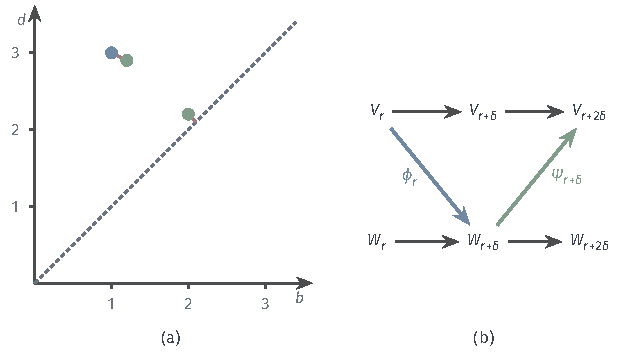
\includegraphics[width=105.184mm]{figures/04-spaces-measures-and-geometry/04-manifolds/tikz/mrec-diagram/figure.pdf}
  \caption{持久图的匹配与持久模的交错。(a) 例~\ref{ex:mrec-bottleneck}的两张持久图，$D_1$为蓝点，$D_2$为绿点，红色线段表示最优匹配，靠近对角线的绿点匹配到对角线。(b) 交错的一个片段：先走蓝色的$\phi$，再走绿色的$\psi$，结果等于沿$V$直接走$2\delta$。}
  \label{fig:mrec-diagram}
\end{BookInlineFigure}

\subsection{过滤交错}
\label{sec:mrec-interleaving}

现在比较同一组点标签上的两张距离表。设$d=[d_{i,j}]$与$d'=[d'_{i,j}]$都是对称、零对角的非负矩阵，可以来自同一组点在两次测量中的结果，并且$\lvert d_{i,j}-d'_{i,j}\rvert\leq\delta$对所有$i,j$成立。记$R_r(d)$为按距离表$d$、直径界$r$构造的Rips复形。

若$\sigma$在$R_r(d)$中，它的每对顶点满足$d_{i,j}\leq r$，从而$d'_{i,j}\leq r+\delta$，所以$\sigma$在$R_{r+\delta}(d')$中。对称地，$R_r(d')\subseteq R_{r+\delta}(d)$。于是两套过滤交替地相互包含：
\begin{equation}
 R_r(d)\subseteq R_{r+\delta}(d')\subseteq R_{r+2\delta}(d),
 \label{eq:mrec-rips-interleave-1}
\end{equation}
\begin{equation}
 R_r(d')\subseteq R_{r+\delta}(d)\subseteq R_{r+2\delta}(d').
 \label{eq:mrec-rips-interleave-2}
\end{equation}

这些复形都是同一个顶点集上全体单纯形的子复形，所有映射都是包含，所以复合的包含$R_r(d)\subseteq R_{r+2\delta}(d)$与原过滤中的推进是同一个包含，与沿过滤推进再平移的各种路径都相容。把这种“隔一步能互相换过去、并且与自身的推进相容”的关系抽象出来，就是下面的定义。

\begin{definition}[交错]
\label{def:mrec-interleaving}
设$\{V_r,v_{r,r'}\}$与$\{W_r,w_{r,r'}\}$是两个持久模，$\delta\geq0$。若存在线性映射$\phi_r:V_r\to W_{r+\delta}$与$\psi_r:W_r\to V_{r+\delta}$，它们与两个持久模自身的映射交换，并满足$\psi_{r+\delta}\circ\phi_r=v_{r,r+2\delta}$与$\phi_{r+\delta}\circ\psi_r=w_{r,r+2\delta}$，则称两个持久模$\delta$\term{交错}（interleaved）。
\end{definition}

图~\ref{fig:mrec-diagram}(b)画的是其中一个等式：沿蓝、绿两条斜线走到$V_{r+2\delta}$，与沿上面一行直接走是同一个映射。对两套Rips过滤取$k$维同调，式~\eqref{eq:mrec-rips-interleave-1}和式~\eqref{eq:mrec-rips-interleave-2}的包含诱导出$\phi_r$与$\psi_r$；包含的复合等于包含，诱导映射的复合也就等于诱导映射，定义中的等式全部成立。所以两个持久模$\delta$交错。

交错为什么能控制条形码？下面的不等式给出最直接的一步。

\begin{lemma}[秩的比较]
\label{lem:mrec-rank-interleaving}
设两个持久模$\delta$交错，$r+2\delta\leq r'$，则
\begin{equation}
 \operatorname{rank}v_{r,r'}\leq\operatorname{rank}w_{r+\delta,r'-\delta}.
 \label{eq:mrec-rank-interleaving}
\end{equation}
\end{lemma}
\begin{proof}
由交错的定义，$v_{r,r'}$可以分解为
\[
 V_r\xrightarrow{\ \phi_r\ }W_{r+\delta}\xrightarrow{\ w\ }W_{r'-\delta}\xrightarrow{\ \psi_{r'-\delta}\ }V_{r'} .
\]
事实上，$\phi$与两个持久模自身的映射交换，所以
\[
 w_{r+\delta,r'-\delta}\circ\phi_r=\phi_{r'-2\delta}\circ v_{r,r'-2\delta}.
\]
再用交错定义中的等式，
\[
 \psi_{r'-\delta}\circ\phi_{r'-2\delta}=v_{r'-2\delta,r'} ,
\]
就得到$v_{r,r'}$。复合映射的秩不超过中间映射的秩。
\end{proof}

由区间分解后的计数，式~\eqref{eq:mrec-rank-interleaving}说：$V$中覆盖$[r,r']$的条的根数，不超过$W$中覆盖$[r+\delta,r'-\delta]$的条的根数。这正是“一根条在对方那里有一根端点相差不超过$\delta$的对应条”的计数形式。把这些计数不等式对所有$r,r'$合起来，再用组合匹配的论证，就能得到下面的定理。

\begin{theorem}[持久图的稳定性]
\label{thm:mrec-stability}
设两个持久模的每个空间都是有限维的，并且它们$\delta$交错，则它们的持久图的瓶颈距离不超过$\delta$。特别地，若两张距离表逐项之差不超过$\delta$，则对每个$k$，两套Rips过滤的$k$维持久图满足$d_B\leq\delta$。
\end{theorem}

这一结果称为代数稳定性定理，从计数不等式到匹配的证明较长，读者可查阅Chazal等人关于持久模稳定性的论文。

它的作用是把几何上的扰动换成表示上的扰动。例如每个点移动不超过$\eta$，成对距离至多改变$2\eta$，持久图在瓶颈距离下至多移动$2\eta$。长于$4\eta$的条不会因此消失，只是端点稍有移动；短于这个量的条则可能出现或消失。

定理控制的只是表示的变化。它说两次测量得到的持久图相近，却没有说任何一张持久图反映了底层流形的同调：两张距离表都可能来自采样不足的数据，它们的条形码彼此接近，同时都与流形无关。

\subsection{持久信息的解释}
\label{sec:mrec-persistence-interpretation}

把持久同调与第~\ref{sec:mrec-homology-recovery}节的恢复定理放在一起，可以分清哪些结论有保证。设样本$P\subseteq M$的覆盖精度$\delta_P$满足
\begin{equation}
 2\delta_P<\varepsilon_1<\varepsilon_2<\sqrt{3/5}\,\tau ,
 \label{eq:mrec-recovery-window}
\end{equation}
则区间$[\varepsilon_1,\varepsilon_2]$中的每个$\varepsilon$都满足定理~\ref{thm:mrec-homology-recovery}的条件，称它为恢复窗口。

\paragraph{窗口内的条}

对窗口中的$\varepsilon\leq\varepsilon'$，包含$j:U_\varepsilon\hookrightarrow U_{\varepsilon'}$是同伦等价。理由如下：记$i:M\hookrightarrow U_\varepsilon$、$i':M\hookrightarrow U_{\varepsilon'}$，二者都是同伦等价，且$j\circ i=i'$；取$i$的同伦逆$h$，则
\[
 j\simeq j\circ i\circ h=i'\circ h,
\]
是同伦等价的复合。所以$H_k(U_\varepsilon)\to H_k(U_{\varepsilon'})$是同构。

进一步可以证明，神经引理中的同伦等价能与包含相容地选取，这要求把神经引理的证明做成对包含自然的形式，读者可查阅Chazal与Oudot关于持久性重建的论文。于是Čech过滤在窗口内的诱导映射都是同构。由区间分解，没有区间的端点落在窗口内部，凡是与窗口相交的条都横跨整个窗口，并且这样的$k$维条恰有$\beta_k(M)$根。这是已经建立了恢复保证的结论。

单位圆上$24$个等距样本的例子可以把这件事算到底。条件给出窗口$\varepsilon_1=2\delta_P\approx0.262$到$\varepsilon_2\approx0.775$。Čech过滤中，相邻两球在$r$超过弦长的一半$\approx0.131$时相交，圆环在此形成；圆心在$r$超过$1$时才被覆盖。所以$H_1$唯一的条是$(0.131,1]$，它横跨窗口，根数$1=\beta_1(S^1)$；$H_0$除了永不消失的条，$23$根短条都在$0.131$处结束，在窗口之前，见图~\ref{fig:mrec-barcodes}(c)。

\paragraph{窗口外的条}

窗口外的条没有这样的保证。很靠近$0$的短条通常反映采样的离散性，很大尺度上的条则反映样本整体的粗略形状，它们与$M$的关系都没有经过论证。更重要的是，实际中并不知道$\delta_P$和$\tau$，也就不知道窗口在哪里，甚至不知道窗口是否存在。

没有覆盖、噪声和几何尺度的条件时，寿命长只表示同调类跨越很大的尺度范围而持续存在。一个例子是：底层集合是一个实心圆盘，没有洞，但样本只取在它的边界圆附近。Rips过滤会给出一根很长的一维条，它如实地反映了样本的形状，却不是圆盘的孔洞；问题出在样本没有覆盖圆盘内部，任何对持久图的处理都无法补上未被采样的区域。

\paragraph{其他过滤与噪声}

上面的结论是对样本在流形上的Čech过滤建立的。对Rips过滤，只能借助式~\eqref{eq:mrec-cech-rips}的夹逼关系，把恢复窗口中的信息传过来，这要求窗口跨越一倍以上的尺度，需要另行论证；正六边形的$H_2$条提醒我们，Rips过滤确实可能给出流形中不存在的同调。观测离开流形时，恢复窗口本身需要重新建立。

表示的稳定性也不能单独证明真实孔洞的存在：定理~\ref{thm:mrec-stability}保证小扰动不会让长条消失，但长条从哪里来，要由覆盖、噪声和可达半径的条件回答。持久同调提供的是跨尺度的完整记录及其稳定性，它与恢复保证配合使用，不能替代后者。

\section{本章小结}
\label{sec:mrec-summary}

本章开头问：只凭有限个样本，能否知道一个未知流形在各点朝哪个方向、局部长什么样、沿它走有多远、有几个分支和几个洞。回答的前提是一个共同的采样模型。覆盖精度说明流形上有没有远离样本的地方，扰动界说明观测离开流形多远，可达半径同时度量流形在环境中的弯曲以及不同部分相互接近的程度，并保证不同分支至少相隔$2\tau$。这些量是分析的假设，不能从样本中准确读出；全域稠密也不保证每个邻域内样本在各切向上都有展开。

可达半径有两条局部推论。半径为$\tau$的球能贴着流形滚动，由此得到流形偏离切平面的二次界；对弦的中点反复投影，得到内在距离与弦长的比较。后面每一节都用到它们。

局部几何的恢复建立在切向近似上。局部PCA用邻域协方差的主方向估计切空间，它最小化到子空间的平方距离和；把弯曲与扰动写进协方差的扰动，由谱隙界得到方向误差，弯曲项随邻域半径增大、噪声项随半径减小，两者都依赖样本在切向上的展开程度。在估计的平面上用含常数项、一次项与二次项的多项式拟合法向分量，就得到连续的局部片；函数值误差不控制导数，多片的并也不自动是流形。

内在距离由邻域图上的最短路逼近。只要覆盖精度小于半径的一半、半径小于$2\tau$，图距离与内在距离之比就夹在两个因子之间，分别由$r/\tau$与$\delta/r$决定。缺采样使图距离过大甚至断开，邻接过大使它跨越相近的部分而过小，离开流形的噪声还要求半径明显大于扰动界。

拓扑的恢复走另一条路，不依赖局部拟合。样本的球并把离散点变成连续空间，Čech复形是它的神经，有限欧氏开球构成良覆盖，神经引理使二者同伦等价，同调随之可以由边界矩阵算出。在样本$\varepsilon/2$稠密且$\varepsilon<\sqrt{3/5}\,\tau$时，每一点沿直线推向最近点的路径留在球并内，球并形变收缩到流形。这恢复的是同调，不是同胚；样本离开流形或改用Rips复形都需要另行论证。

尺度未知时，持久同调让复形随尺度增长，用包含诱导的映射追踪同调类，有限过滤的持久模分解为区间，得到条形码与持久图。两张距离表逐项相差不超过$\delta$时，两套Rips过滤$\delta$交错，持久图的瓶颈距离不超过$\delta$，这是表示的稳定性。只有在恢复窗口内，横跨窗口的条才对应流形的同调；寿命长只说明跨尺度持续，不能单独证明真实孔洞的存在。

表~\ref{tab:mrec-summary}把各条线索的输入、关键条件和输出列在一起，它们各有自己的条件和结论，不能相互替代。

\begin{BookInlineTable}
  \centering
  \caption{本章各线索的条件与结论}
  \label{tab:mrec-summary}
  \begin{tabular}{lll}
    \toprule
    线索 & 关键条件 & 结论 \\
    \midrule
    切空间估计 & $\lambda_T>0$，$\beta$相对$\lambda_T$小 & 方向误差~\eqref{eq:mrec-local-pca-error} \\
    局部片拟合 & $\bm\Phi$满列秩，图表示成立 & 系数误差~\eqref{eq:mrec-coefficient-error} \\
    内在距离 & $2\delta<r<2\tau$ & 比值界~\eqref{eq:mrec-graph-lower}、\eqref{eq:mrec-graph-upper} \\
    同调恢复 & $\varepsilon/2$稠密，$\varepsilon<\sqrt{3/5}\,\tau$ & 同构~\eqref{eq:mrec-homology-recovery} \\
    持久图稳定性 & 距离表逐项相差不超过$\delta$ & $d_B\leq\delta$ \\
    \bottomrule
  \end{tabular}
\end{BookInlineTable}

本章的条件都是确定性的：给定样本与扰动界，判断结论是否成立。样本随机抽取时这些条件以多大概率满足，属于卷八的统计问题；以拟合残差或距离畸变为目标的进一步优化，则属于卷五。

